%%
%% Supplementary Material for SalientGS
%% ACM Multimedia 2026
%%
\documentclass[sigconf]{acmart}

\usepackage{multirow}
\usepackage{colortbl}
\usepackage{booktabs}
% The local validation environment lacks the ACM font bundle; disable
% expansion only for that fallback. TAPS supplies the official fonts.
\IfFileExists{libertine.sty}{}{\microtypesetup{expansion=false}}
\graphicspath{{./}{samples/}}
\definecolor{tabfirst}{rgb}{1, 0.6, 0.6} % red
\definecolor{tabsecond}{rgb}{1, 0.8, 0.5} % orange
\definecolor{tabthird}{rgb}{1, 1, 0.6} % yellow

%% ACM Multimedia 2026 Conference Information (match main paper header)
\acmConference[ACM MM '26]{ACM Multimedia 2026}{November 10--14, 2026}{Rio de Janeiro, Brazil }

%% Suppress ACM reference/copyright blocks for supplementary
\settopmatter{printacmref=false}
\renewcommand\footnotetextcopyrightpermission[1]{}
\pagestyle{plain}

\begin{document}
\setlength{\emergencystretch}{2em}

\title{SalientGS: Supplementary Material}

\author{Tianyu Xiong}
\affiliation{%
  \institution{School of Computer Science, Northwestern Polytechnical University}
  \city{Xi'an}
  \country{China}
}
\author{Rui Li}
\affiliation{%
  \institution{CEMSE, King Abdullah University of Science and Technology}
  \city{Thuwal}
  \country{Saudi Arabia}
}
\author{Suning Ge}
\affiliation{%
  \institution{School of Computer Science, Northwestern Polytechnical University}
  \city{Xi'an}
  \country{China}
}
\author{Jiaqi Yang}
\affiliation{%
  \institution{School of Computer Science, Northwestern Polytechnical University}
  \city{Xi'an}
  \country{China}
}

\renewcommand{\shortauthors}{T. Xiong et al.}

\maketitle

\section{Overview}

This supplementary material accompanies the main paper \emph{``SalientGS: Unified SfM-to-3DGS with Importance-Guided MCMC Gaussian Allocation.''}
We provide:
\begin{itemize}
    \item A released-code cross-benchmark verification with an explicit macro-average protocol (\S\ref{sec:supp_release_verification}).
    \item A large-scene benchmark comparison (\S\ref{sec:supp_large_scene}).
    \item Full SfM runtime tables for the Courthouse scene (\S\ref{sec:supp_runtime}).
    \item Full per-scene qualitative comparisons on all nine Mip-NeRF 360 scenes (\S\ref{sec:supp_qualitative}).
    \item Per-image LPIPS analysis across ablation variants (\S\ref{sec:supp_per_image_lpips}).
    \item Threshold-sensitivity sweeps for $\tau_{\text{imp}}$ and the number of scoring views $K$ (\S\ref{sec:supp_threshold}).
    \item Analysis of the SalientGS front-end: track-length distributions and a controlled track-cap ablation establishing that sufficient multi-view track coverage is a prerequisite for high reconstruction quality (\S\ref{sec:supp_track_analysis}).
\end{itemize}

\section{Released-Code Cross-Benchmark Verification}
\label{sec:supp_release_verification}

Table~\ref{tab:supp_cross_benchmark} macro-averages the three dataset-level entries in the main paper, assigning equal weight to Mip-NeRF 360, Deep Blending, and Tanks \& Temples. This is a cross-dataset summary, not a replacement for the individual benchmark results. Failed scenes remain in the corresponding dataset aggregate; notably, the \textit{drjohnson} failures of GloSplat-A and VGGT-X are included rather than discarded. Under this explicit protocol, SalientGS has the best macro-average quality and runtime in the comparison. Its advantage reflects consistency across datasets: it is the only method with a top-two LPIPS result on every benchmark.

\begin{table}[t]
    \centering
    \footnotesize
    \setlength\tabcolsep{4pt}
    \caption{Cross-benchmark macro-average of the three dataset-level entries in the main comparison. Time is end-to-end minutes; each benchmark receives equal weight.}
    \label{tab:supp_cross_benchmark}
    \begin{tabular}{lrrrr}
        \toprule
        Method & Time$\downarrow$ & PSNR$\uparrow$ & SSIM$\uparrow$ & LPIPS$\downarrow$ \\
        \midrule
        3DGS & 28.35 & 26.98 & 0.855 & 0.211 \\
        3DGS-MCMC & 28.85 & 27.40 & 0.872 & 0.191 \\
        Mini-Splatting & 24.37 & 26.92 & 0.857 & 0.214 \\
        Speedy-splat & 21.15 & 26.57 & 0.832 & 0.270 \\
        Taming-3DGS & 14.71 & 26.96 & 0.840 & 0.251 \\
        DashGaussian & 15.93 & 27.13 & 0.859 & 0.214 \\
        FastGS-big & 13.54 & 27.48 & 0.861 & 0.211 \\
        GloSplat-A & 22.01 & 23.15 & 0.750 & 0.265 \\
        VGGT-X & 64.02 & 22.60 & 0.741 & 0.287 \\
        \textbf{SalientGS} & \textbf{10.62} & \textbf{27.65} & \textbf{0.876} & \textbf{0.147} \\
        \bottomrule
    \end{tabular}
\end{table}

The released per-scene CSV uses seed 42, exactly 30K optimization steps, and a 1.5M Gaussian cap. All 13 runs execute feature extraction, matching, SfM, and training; reference sparse models are not used. For Mip-NeRF 360, the scene-equal aggregate used in the main comparison is 28.822 / 0.853 / 0.148 (PSNR / SSIM / LPIPS). Pooling all held-out images instead gives 29.607 / 0.874 / 0.140 because scenes contain different numbers of test images. We report the latter only as a diagnostic and never compare it against scene-averaged baselines.

\begin{table*}[t]
    \centering
    \footnotesize
    \setlength\tabcolsep{5pt}
    \caption{Released-code verification by scene. Time includes feature extraction, matching, SfM, and 30K-step training on one RTX PRO 6000 Blackwell GPU. Every final model contains 1.5M Gaussians.}
    \label{tab:supp_release_per_scene}
    \begin{tabular}{llrrrr}
        \toprule
        Dataset & Scene & PSNR$\uparrow$ & SSIM$\uparrow$ & LPIPS$\downarrow$ & Time (min)$\downarrow$ \\
        \midrule
        \multirow{9}{*}{Mip-NeRF 360}
        & bicycle & 27.125 & 0.828 & 0.135 & 10.37 \\
        & bonsai & 33.207 & 0.955 & 0.106 & 13.53 \\
        & counter & 29.604 & 0.919 & 0.136 & 14.03 \\
        & flowers & 22.826 & 0.661 & 0.274 & 10.48 \\
        & garden & 29.188 & 0.894 & 0.074 & 10.33 \\
        & kitchen & 32.786 & 0.943 & 0.076 & 13.57 \\
        & room & 31.945 & 0.928 & 0.150 & 12.72 \\
        & stump & 28.310 & 0.836 & 0.123 & 10.86 \\
        & treehill & 24.407 & 0.714 & 0.260 & 10.20 \\
        \midrule
        \multirow{2}{*}{Deep Blending}
        & drjohnson & 28.824 & 0.892 & 0.210 & 10.69 \\
        & playroom & 30.153 & 0.920 & 0.156 & 9.39 \\
        \midrule
        \multirow{2}{*}{Tanks \& Temples}
        & train & 23.003 & 0.846 & 0.128 & 10.32 \\
        & truck & 26.306 & 0.893 & 0.090 & 9.73 \\
        \bottomrule
    \end{tabular}
\end{table*}

%% =============================================================================
%% Large-Scene Benchmark Comparison
%% =============================================================================
\section{Large-Scene Benchmark Comparison}
\label{sec:supp_large_scene}


\begin{table*}[t]
    \centering
    % \scriptsize
    % \setlength\tabcolsep{3pt}
    \caption{
        \textbf{Large-scene benchmark comparison.}
        Metrics are SSIM$\uparrow$, PSNR$\uparrow$, and LPIPS$\downarrow$. Red / orange / yellow denote the best / second-best / third-best values in each column.
    }
    \resizebox{\textwidth}{!}{%
    \begin{tabular}{lcccccccccccc}
        \toprule
        & \multicolumn{3}{c}{Building} & \multicolumn{3}{c}{Rubble} & \multicolumn{3}{c}{Residence} & \multicolumn{3}{c}{Sci-Art} \\
        \cmidrule(lr){2-4} \cmidrule(lr){5-7} \cmidrule(lr){8-10} \cmidrule(lr){11-13}
        Method & SSIM & PSNR & LPIPS & SSIM & PSNR & LPIPS & SSIM & PSNR & LPIPS & SSIM & PSNR & LPIPS \\
        \midrule
        \multicolumn{13}{l}{\textit{w/ Geometric Optimization}} \\
        SuGaR~\cite{sugar2024}
            & 0.507 & 17.76 & 0.455
            & 0.577 & 20.69 & 0.453
            & 0.603 & 18.74 & 0.406
            & 0.698 & 18.60 & 0.349 \\
        NeuS~\cite{wang2021neus}
            & 0.463 & 18.01 & 0.611
            & 0.480 & 20.46 & 0.618
            & 0.503 & 17.85 & 0.533
            & 0.633 & 18.62 & 0.472 \\
        Neuralangelo~\cite{li2023neuralangelo}
            & 0.582 & 17.89 & 0.322
            & 0.625 & 20.18 & 0.314
            & 0.644 & 18.03 & 0.263
            & 0.769 & 19.10 & 0.231 \\
        PGSR~\cite{chen2024pgsr}
            & 0.480 & 16.12 & 0.573
            & 0.728 & 23.09 & 0.334
            & 0.746 & 20.57 & 0.289
            & 0.799 & 19.72 & 0.275 \\
        VCR-Gaus~\cite{vcrgaus2024}
            & 0.502 & 19.56 & 0.502
            & 0.541 & 21.34 & 0.428
            & 0.623 & 20.59 & 0.359
            & 0.665 & 19.31 & 0.465 \\
        CityGaussianV2~\cite{liu2025citygaussianv2}
            & 0.650 & 19.07 & 0.397
            & 0.720 & 23.75 & 0.322
            & 0.769 & 21.15 & 0.234
            & 0.810 & 20.66 & 0.266 \\
        UrbanGS~\cite{urbangs}
            & \cellcolor{tabthird}0.802 & \cellcolor{tabsecond}22.82 & 0.208
            & 0.791 & \cellcolor{tabsecond}26.25 & \cellcolor{tabfirst}\bf 0.210
            & \cellcolor{tabfirst}\bf 0.823 & \cellcolor{tabthird}22.48 & \cellcolor{tabthird}0.205
            & 0.824 & 22.62 & 0.279 \\
        CityGS-X~\cite{gao2025citygsx}
            & \cellcolor{tabfirst}\bf 0.817 & \cellcolor{tabthird}22.76 & \cellcolor{tabsecond}0.191
            & \cellcolor{tabsecond}0.823 & \cellcolor{tabthird}26.15 & \cellcolor{tabfirst}\bf 0.210
            & \cellcolor{tabsecond}0.819 & 22.44 & \cellcolor{tabsecond}0.194
            & \cellcolor{tabfirst}\bf 0.867 & 22.77 & \cellcolor{tabsecond}0.179 \\
        \midrule
        \multicolumn{13}{l}{\textit{w/o Geometric Optimization}} \\
        Mega-NeRF~\cite{turki2022meganerf}
            & 0.547 & 20.92 & 0.454
            & 0.553 & 24.06 & 0.508
            & 0.628 & 22.08 & 0.401
            & 0.770 & \cellcolor{tabsecond}25.60 & 0.312 \\
        Switch-NeRF~\cite{mi2023switchnerf}
            & 0.579 & 21.54 & 0.397
            & 0.562 & 24.31 & 0.478
            & 0.654 & \cellcolor{tabsecond}22.57 & 0.352
            & 0.795 & \cellcolor{tabfirst}\bf 26.51 & 0.271 \\
        VastGaussian~\cite{lin2024vastgaussian}
            & 0.728 & 21.80 & 0.225
            & 0.742 & 25.20 & 0.264
            & 0.699 & 21.01 & 0.261
            & 0.761 & 22.64 & 0.261 \\
        3DGS~\cite{kerbl3Dgaussians}
            & 0.738 & 22.53 & 0.214
            & 0.725 & 25.51 & 0.316
            & 0.745 & 22.36 & 0.247
            & 0.791 & 24.13 & 0.262 \\
        DoGaussian~\cite{chen2024dogs}
            & 0.759 & 22.73 & \cellcolor{tabthird}0.204
            & 0.765 & 25.78 & 0.257
            & 0.740 & 21.94 & 0.244
            & 0.804 & \cellcolor{tabthird}24.42 & \cellcolor{tabthird}0.219 \\
        CityGaussian~\cite{liu2024citygaussian}
            & 0.778 & 21.55 & 0.246
            & \cellcolor{tabthird}0.813 & 25.77 & 0.228
            & \cellcolor{tabthird}0.813 & 22.00 & 0.211
            & \cellcolor{tabthird}0.837 & 21.39 & 0.230 \\
        \midrule
        SalientGS (Ours)
            & \cellcolor{tabsecond}0.804 & \cellcolor{tabfirst}\bf 24.19 & \cellcolor{tabfirst}\bf 0.181
            & \cellcolor{tabfirst}\bf 0.824 & \cellcolor{tabfirst}\bf 26.98 & \cellcolor{tabthird}0.213
            & \cellcolor{tabthird}0.816 & \cellcolor{tabfirst}\bf 22.67 & \cellcolor{tabfirst}\bf 0.193
            & \cellcolor{tabsecond}0.857 & 22.91 & \cellcolor{tabfirst}\bf 0.173 \\
        \bottomrule
    \end{tabular}%
    }
    \label{tab:supp_large_scene}
\end{table*}

Table~\ref{tab:supp_large_scene} reports SSIM, PSNR, and LPIPS on Building, Rubble, Residence, and Sci-Art; each competing method is cited in the first column. Our method achieves the best PSNR on Building, Rubble, and Residence, the best LPIPS on Building, Residence, and Sci-Art, and the best SSIM on Rubble, indicating that the unified SfM-to-3DGS pipeline remains highly competitive even on challenging large-scale scenes.
Under the same large-scene training setup, SalientGS averages only about 1\,h wall-clock training and $\sim$5\,GB peak GPU memory, compared to about 3\,h and $\sim$14\,GB for CityGS-X~\cite{gao2025citygsx}.

%% =============================================================================
%% SfM Runtime Details
%% =============================================================================
\section{SfM Runtime Details}
\label{sec:supp_runtime}

Table~\ref{tab:supp_sfm_runtime} reports the full SfM component runtime on the Courthouse scene with 250--1000 input images, including GloSplat-F (XFeat+LightGlue with retrieval top-5; see \S\ref{sec:supp_track_analysis} for details). These numbers correspond to the trend summarized by Figure~5 in the main paper.

\begin{table}[t]
    \centering
    \footnotesize
    \setlength\tabcolsep{2pt}
    \caption{
        \textbf{SfM runtime comparison (seconds).} We compare the SfM component runtime across different methods on the Courthouse scene with varying numbers of input images. SalientGS combines Fisher Vector retrieval with first-order SfM optimization to achieve significant speedups over traditional and learning-based approaches.
    }
    \resizebox{\columnwidth}{!}{%
    \begin{tabular}{r rrrrrr}
        \toprule
        \# Images & COLMAP & MASt3R & GloSplat-A & VGGT-X & GloSplat-F & SalientGS \\
        \midrule
        250  & 644.6  & 312.2 & 222.2  & 53.9  & 100.2 & \textbf{47.8} \\
        500  & 1165.0 & 638.0 & 408.2  & 113.3 & 191.9 & \textbf{98.0} \\
        750  & 2226.3 & 978.5 & 855.7  & 249.6 & 250.0 & \textbf{138.5} \\
        1000 & 4349.2 & 1308.2 & 1371.3 & 398.9 & 327.8 & \textbf{186.1} \\
        \bottomrule
    \end{tabular}%
    }
    \label{tab:supp_sfm_runtime}
\end{table}

%% =============================================================================
%% Per-Scene Qualitative Comparisons
%% =============================================================================
\section{Per-Scene Qualitative Comparisons}
\label{sec:supp_qualitative}

We present qualitative comparisons on all nine Mip-NeRF 360~\cite{barron2022mip} scenes.
Each figure shows the rendered output from SalientGS (Ours) alongside ablation variants (Vanilla MCMC, Standard ADC, Freeze Poses) and a baseline method, with zoomed crops at the region of maximum LPIPS difference.

\paragraph{Outdoor Scenes.}
Figures~\ref{fig:supp_bicycle}--\ref{fig:supp_treehill} cover the five outdoor scenes.
SalientGS consistently resolves fine-grained texture---foliage, bark, grass---that Vanilla MCMC blurs and Standard ADC can render with color artifacts on most scenes.
The advantage is most pronounced on \textit{stump} and \textit{flowers}, where high-frequency detail benefits most from importance-guided capacity allocation; on \textit{garden}, SalientGS and Standard ADC perform comparably.

\paragraph{Indoor Scenes.}
Figures~\ref{fig:supp_bonsai}--\ref{fig:supp_room} cover the four indoor scenes.
On \textit{counter}, \textit{bonsai}, and \textit{kitchen}, SalientGS outperforms all ablation variants, though the margins are smaller than on outdoor scenes due to simpler geometry and more uniform textures.
On \textit{room}, SalientGS underperforms VGGT-X on flat, textureless surfaces where first-order SfM initialization provides weaker geometric constraints than learned pose estimators (see main paper, Qualitative Results and Conclusion), though it still leads all ablation variants in the per-image LPIPS table.

\begin{figure*}[t]
    \centering
    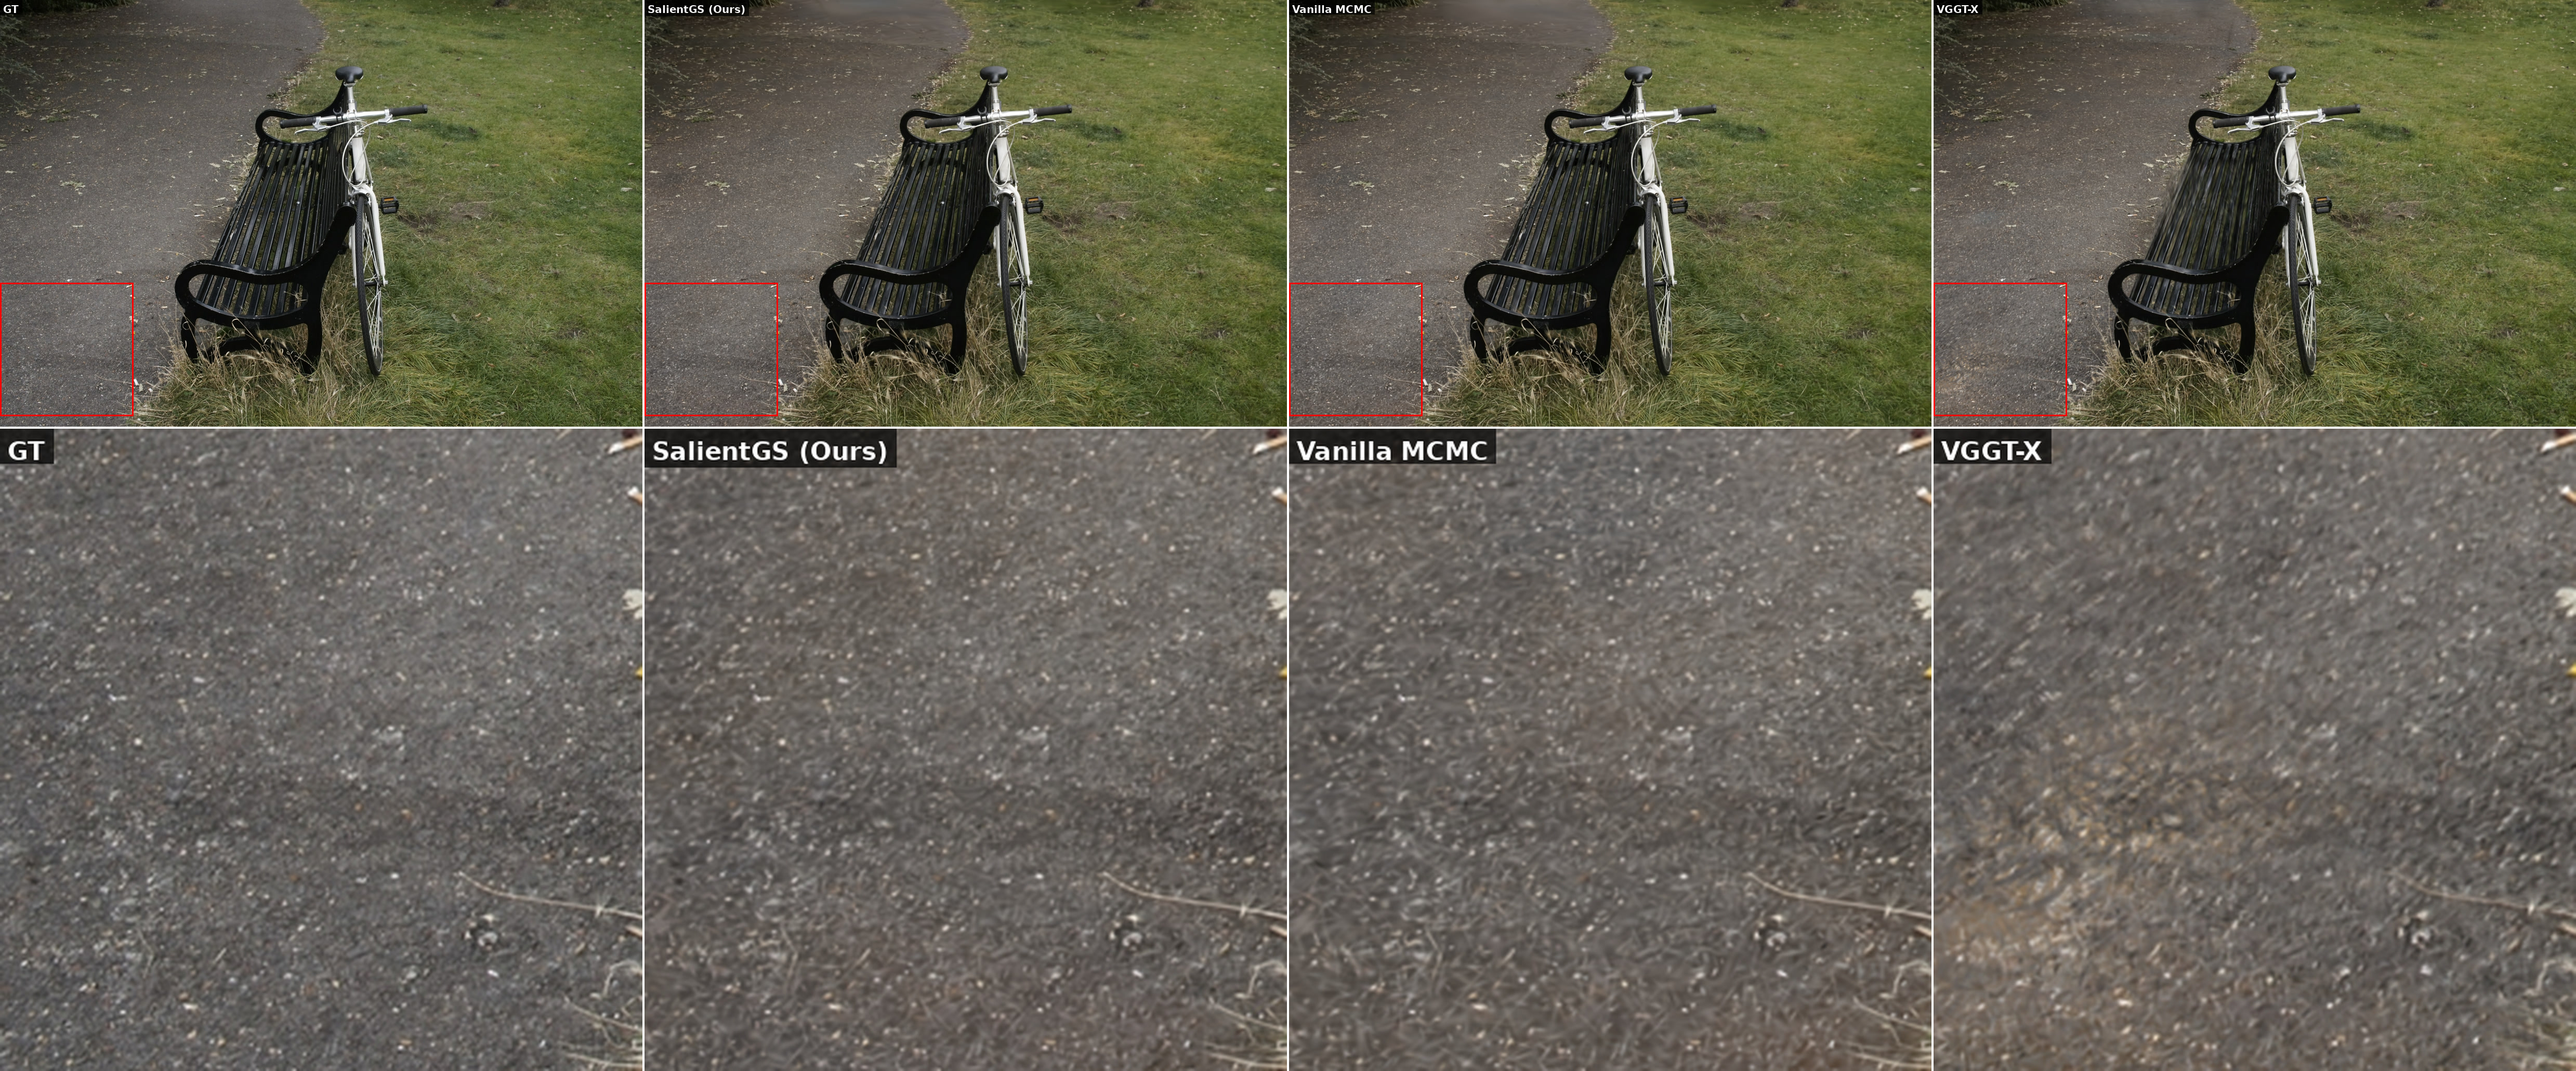
\includegraphics[width=\textwidth]{qualitative/qual_scene_bicycle.jpg}
    \caption{Per-scene qualitative comparison: \textit{bicycle}.}
    \label{fig:supp_bicycle}
\end{figure*}

\begin{figure*}[t]
    \centering
    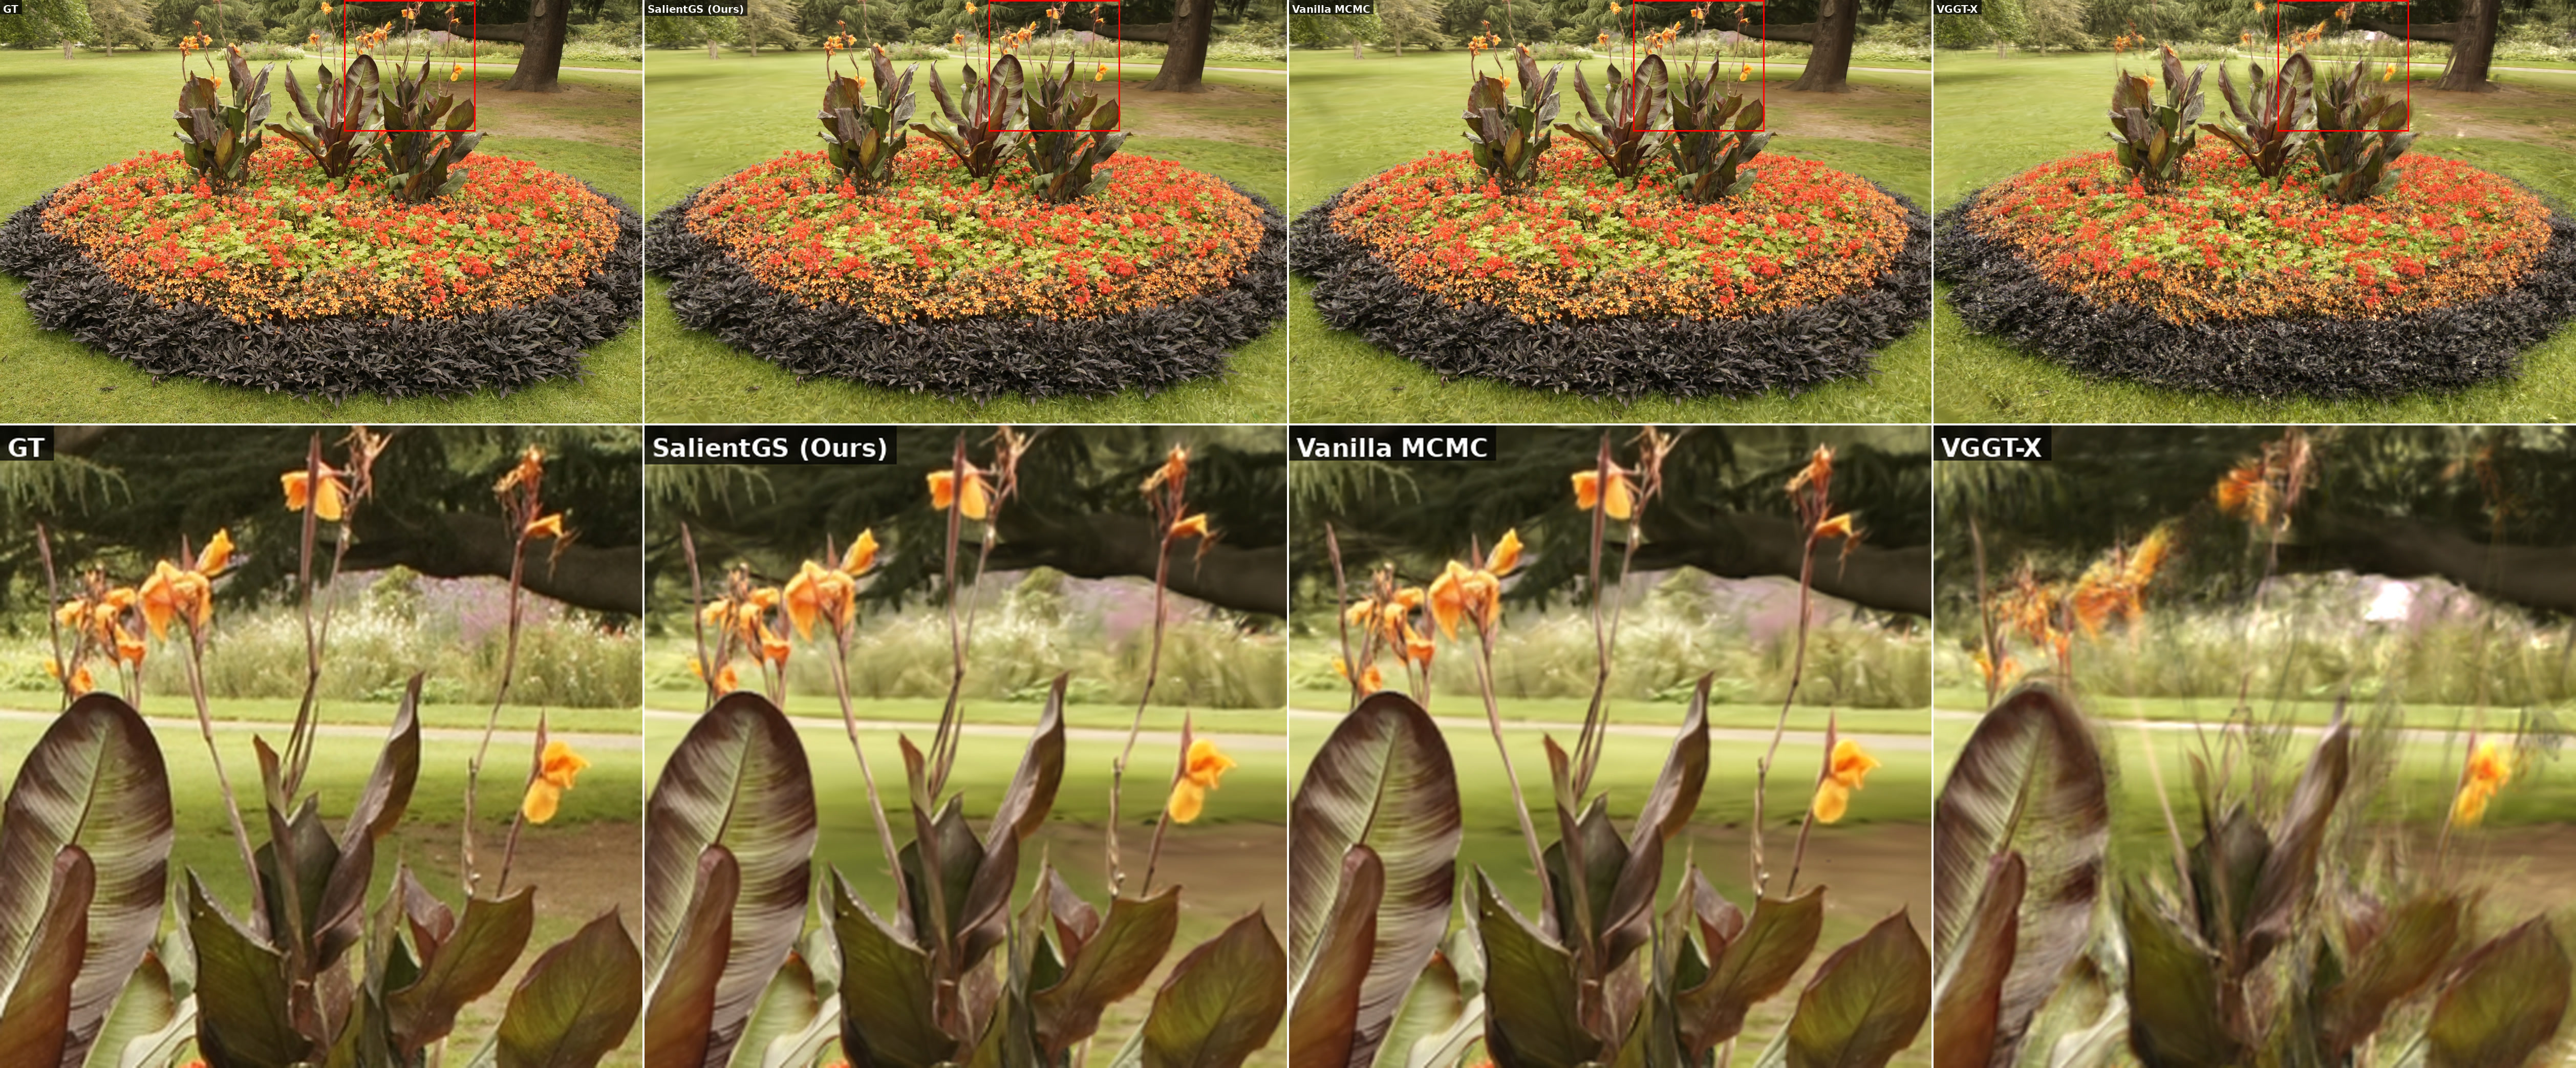
\includegraphics[width=\textwidth]{qualitative/qual_scene_flowers.jpg}
    \caption{Per-scene qualitative comparison: \textit{flowers}.}
    \label{fig:supp_flowers}
\end{figure*}

\begin{figure*}[t]
    \centering
    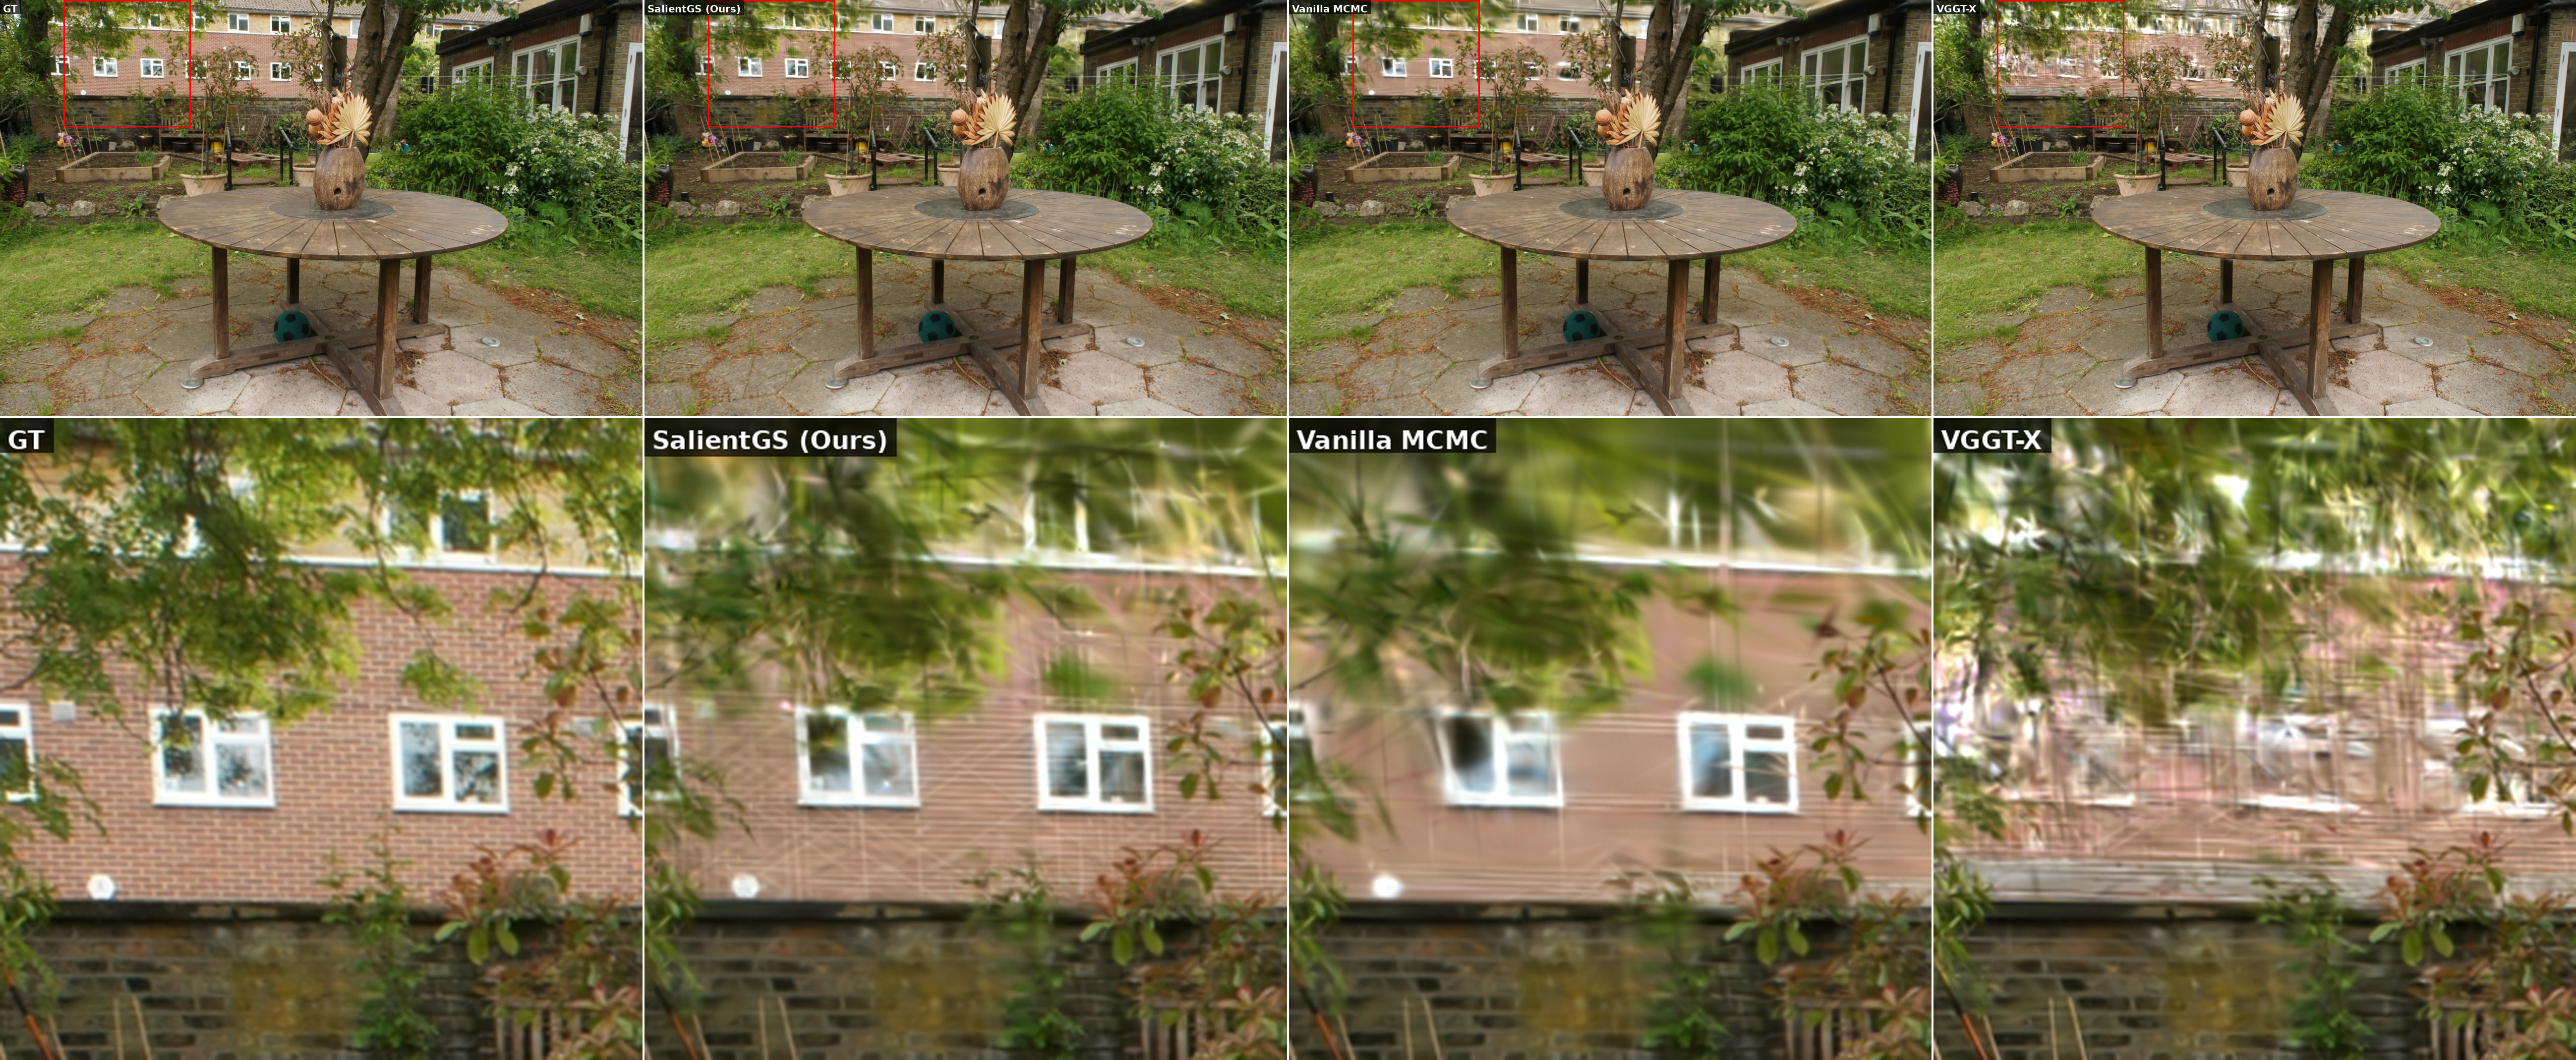
\includegraphics[width=\textwidth]{qualitative/qual_scene_garden.jpg}
    \caption{Per-scene qualitative comparison: \textit{garden}.}
    \label{fig:supp_garden}
\end{figure*}

\begin{figure*}[t]
    \centering
    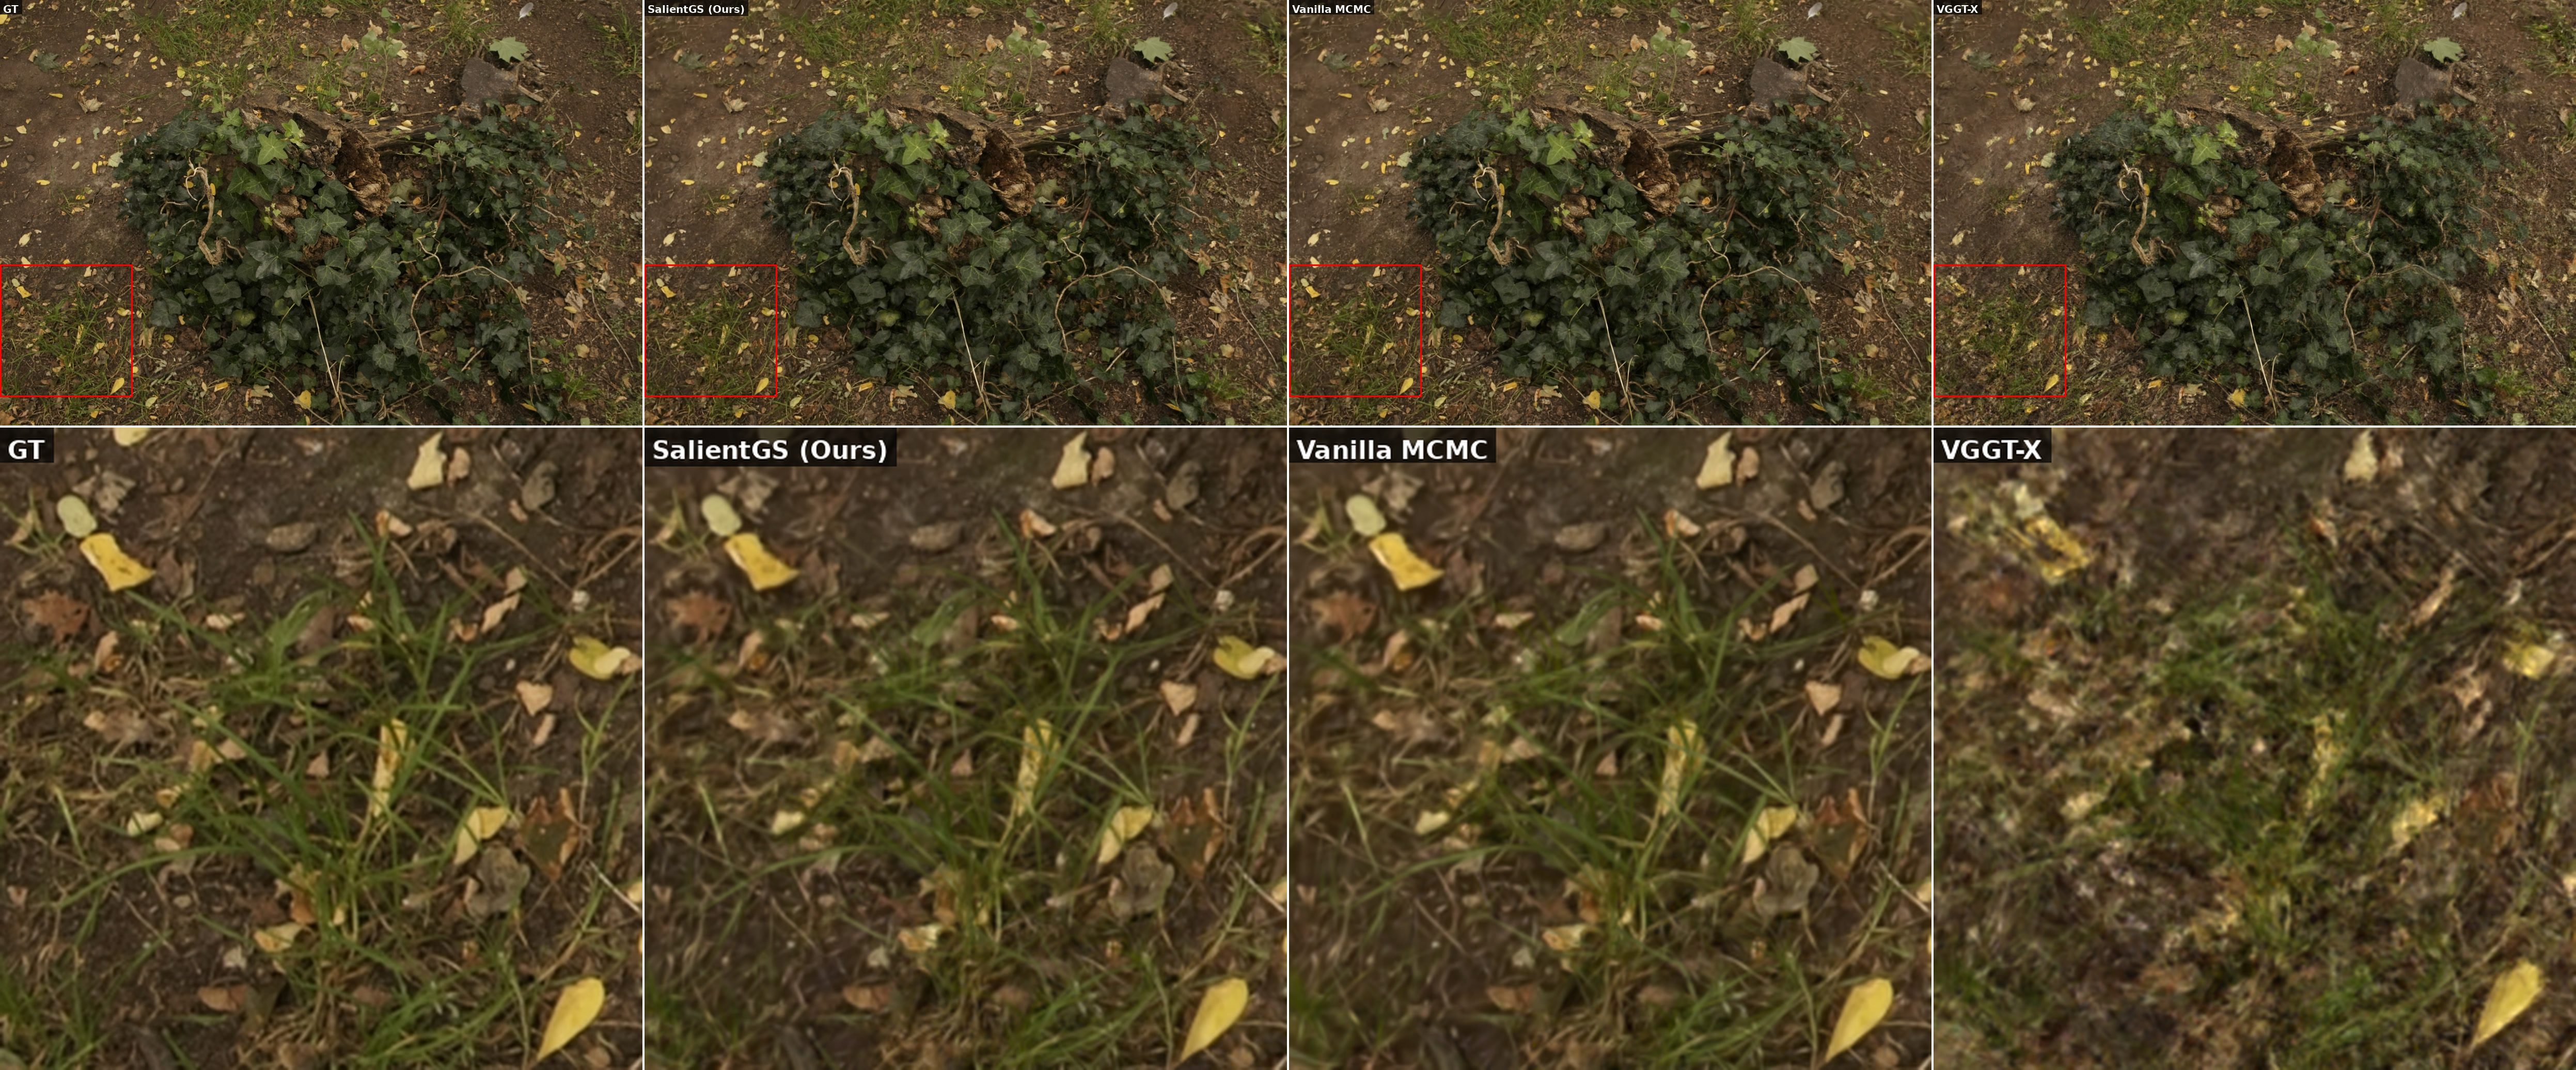
\includegraphics[width=\textwidth]{qualitative/qual_scene_stump.jpg}
    \caption{Per-scene qualitative comparison: \textit{stump}.}
    \label{fig:supp_stump}
\end{figure*}

\begin{figure*}[t]
    \centering
    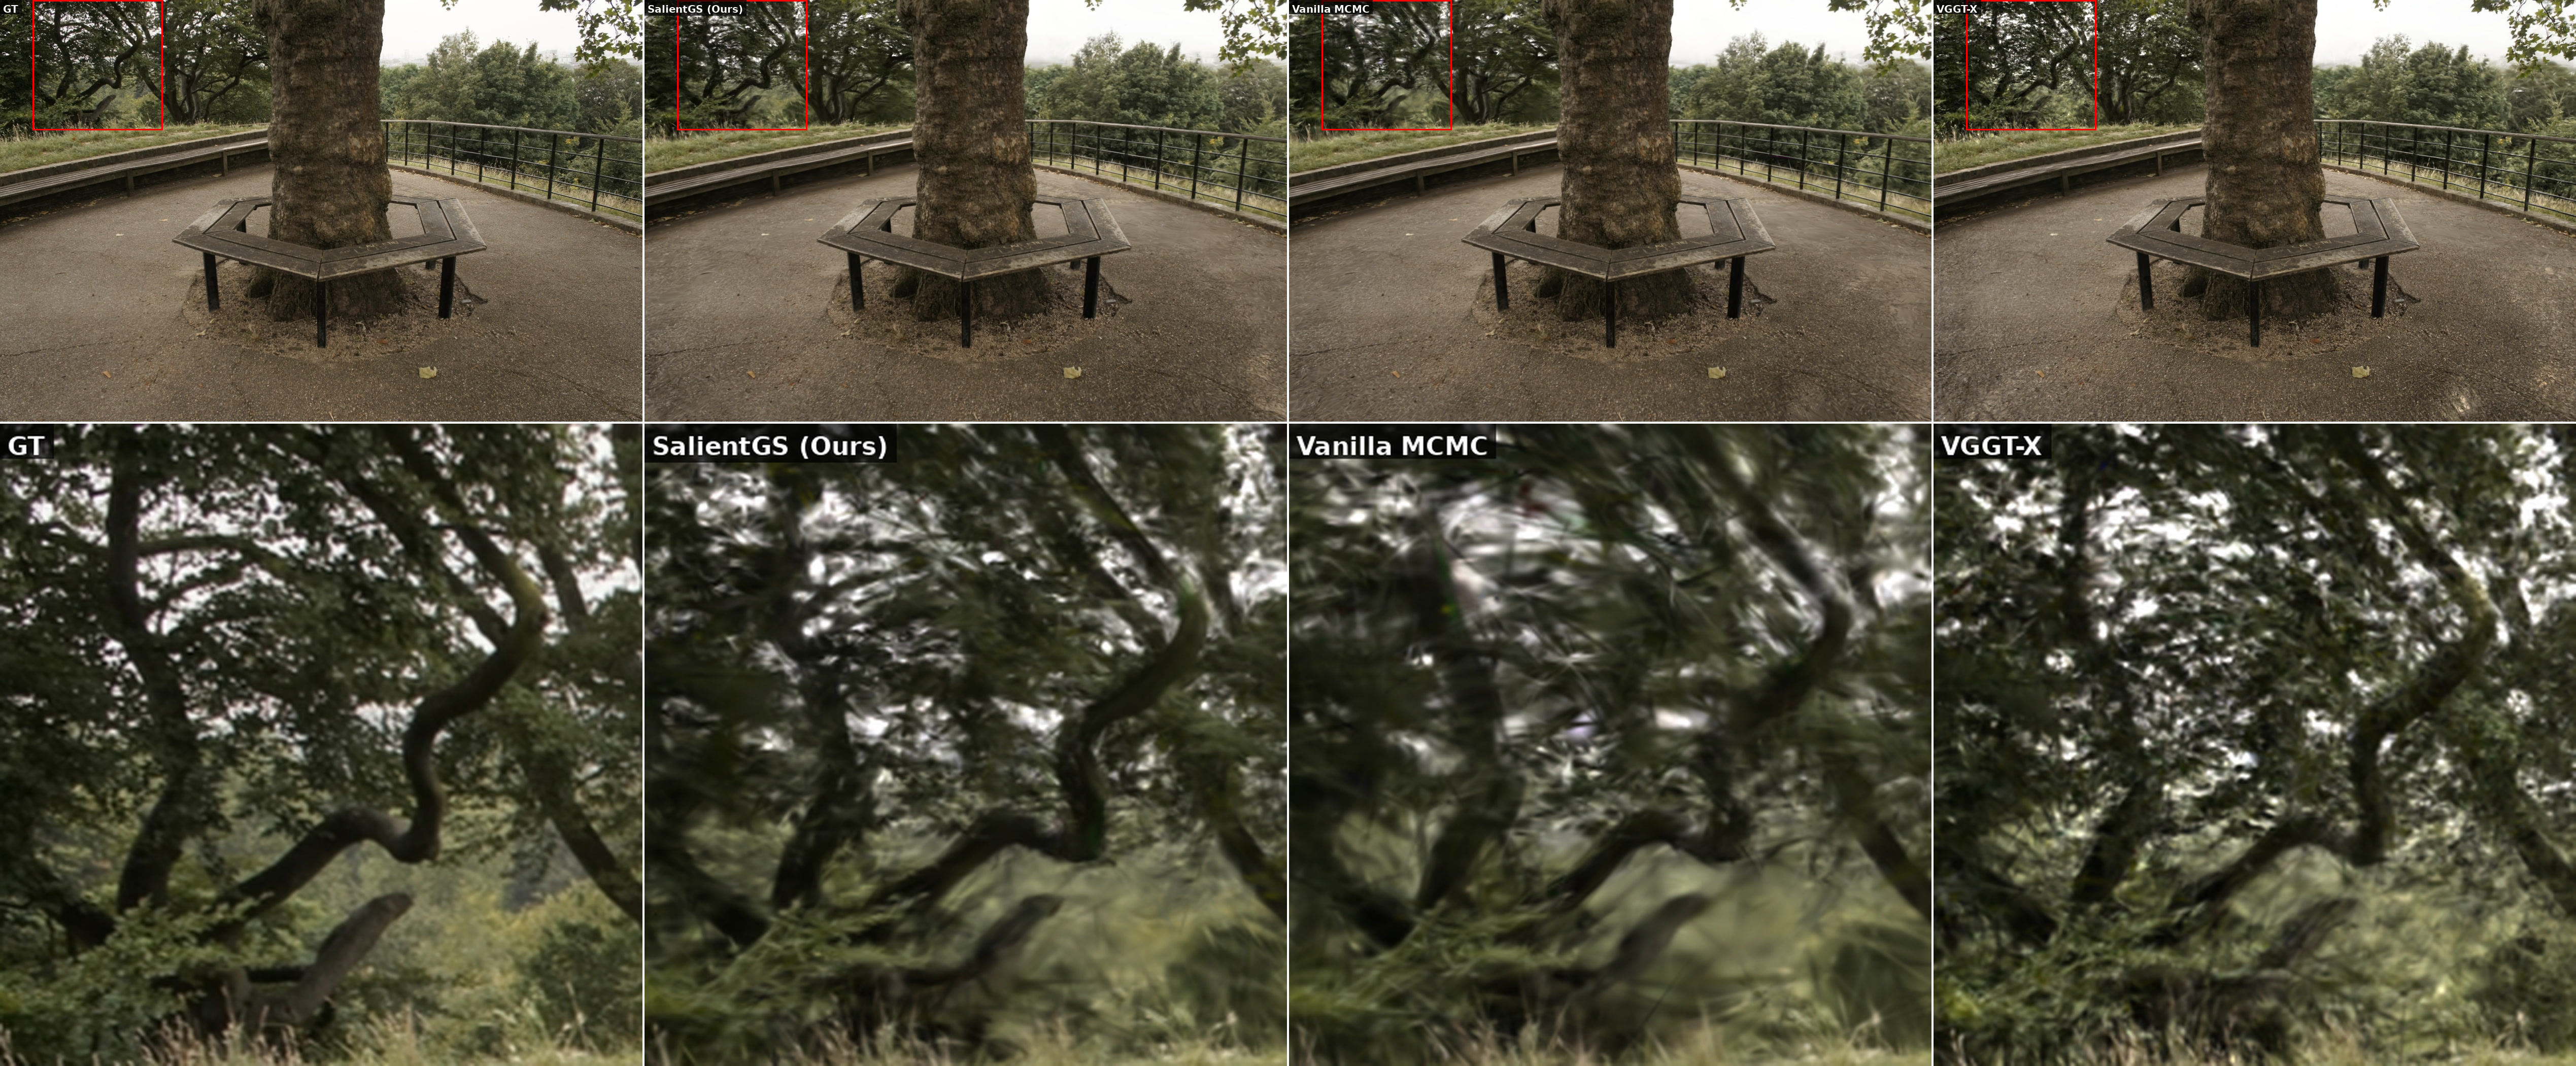
\includegraphics[width=\textwidth]{qualitative/qual_scene_treehill.jpg}
    \caption{Per-scene qualitative comparison: \textit{treehill}.}
    \label{fig:supp_treehill}
\end{figure*}

\begin{figure*}[t]
    \centering
    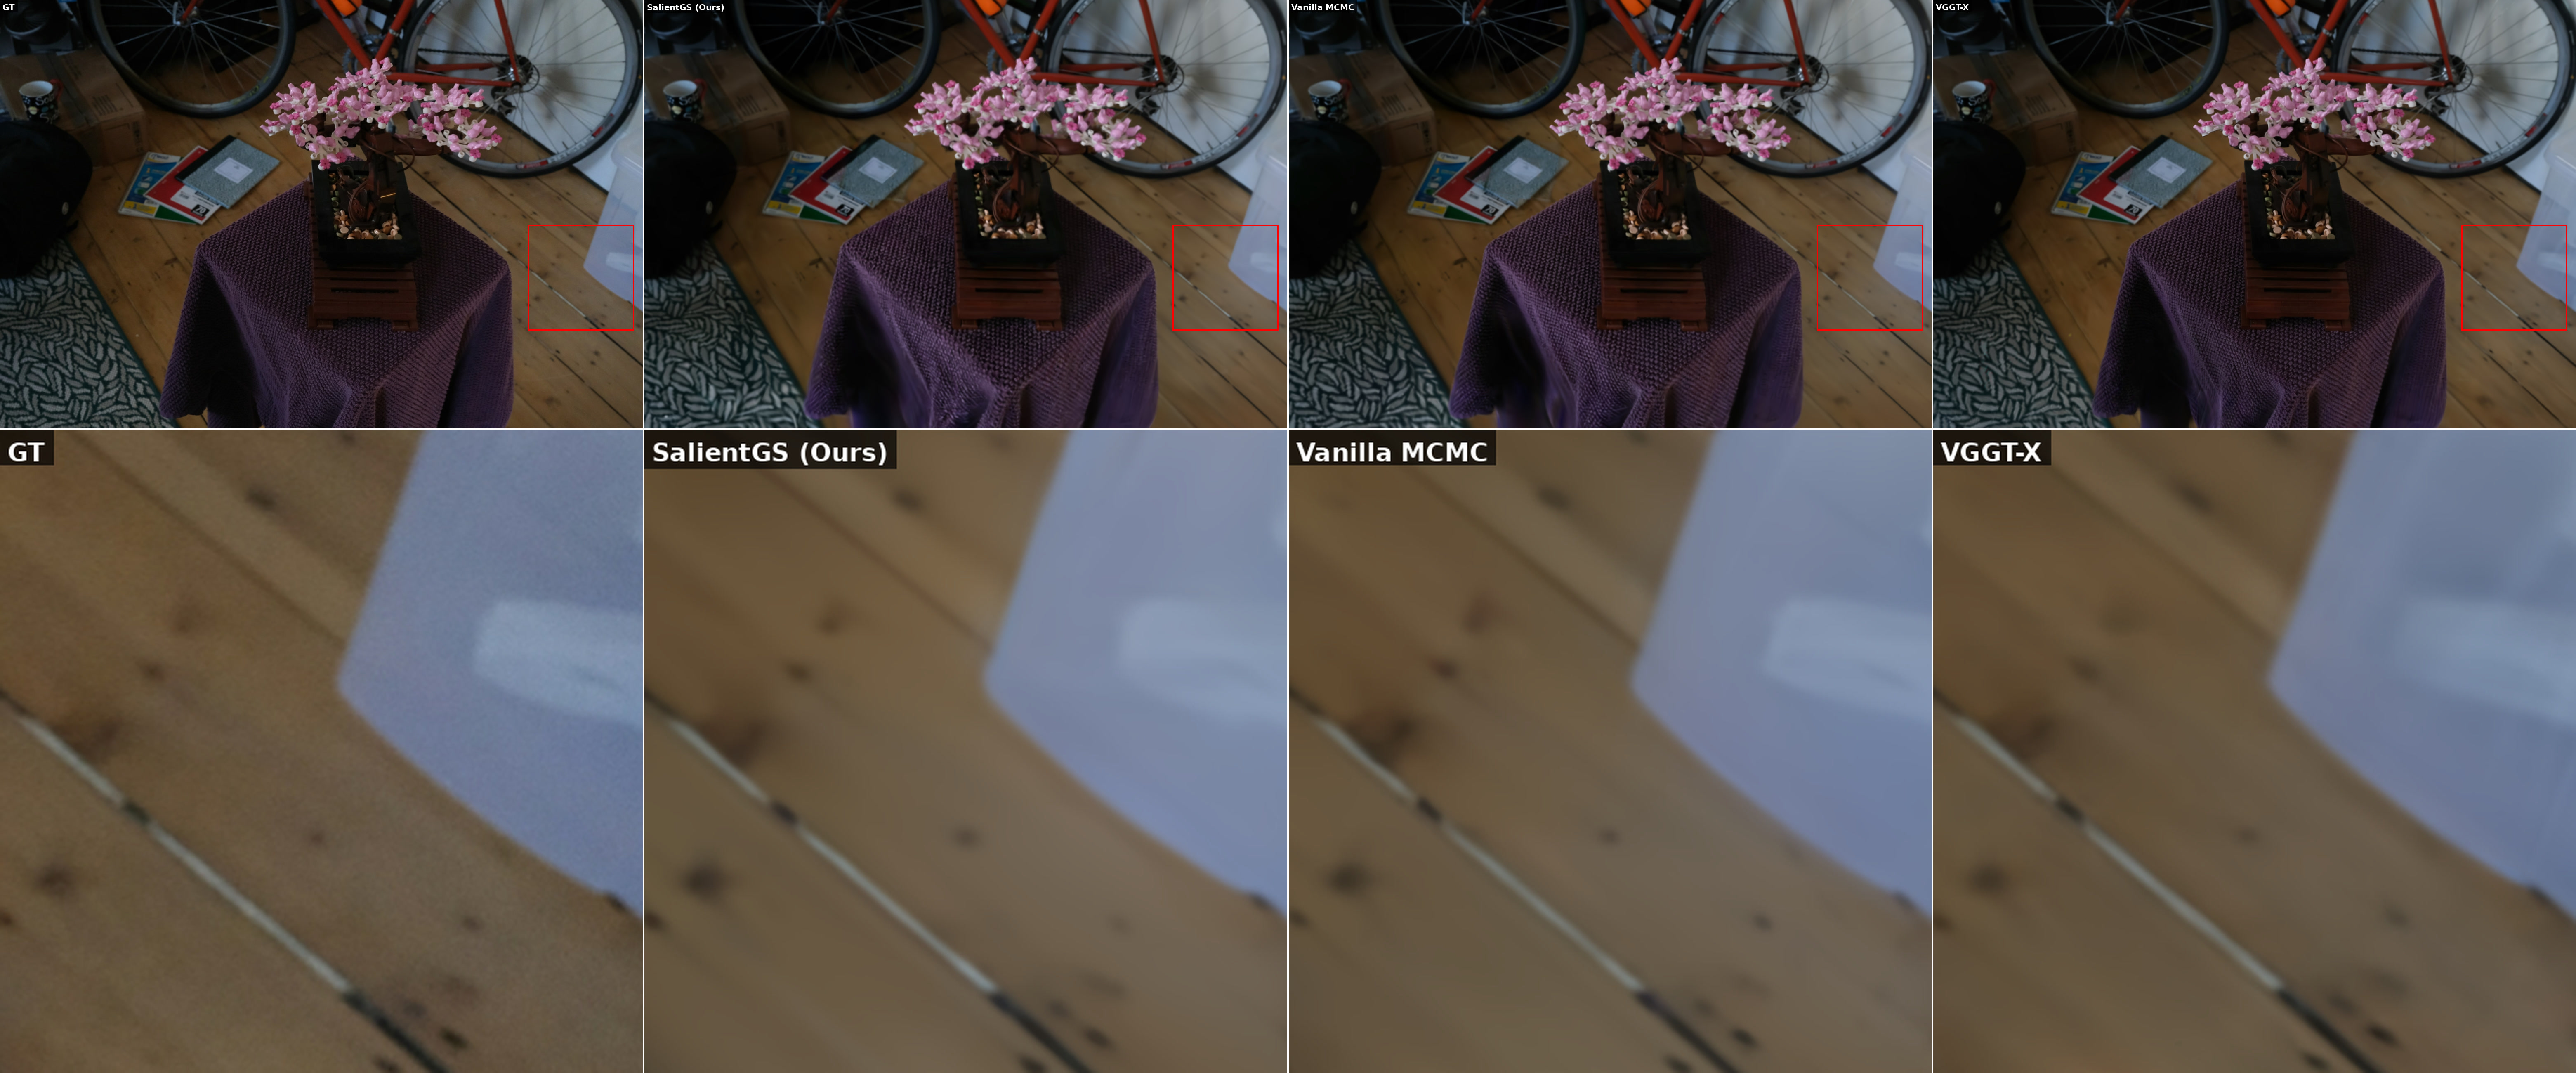
\includegraphics[width=\textwidth]{qualitative/qual_scene_bonsai.jpg}
    \caption{Per-scene qualitative comparison: \textit{bonsai}.}
    \label{fig:supp_bonsai}
\end{figure*}

\begin{figure*}[t]
    \centering
    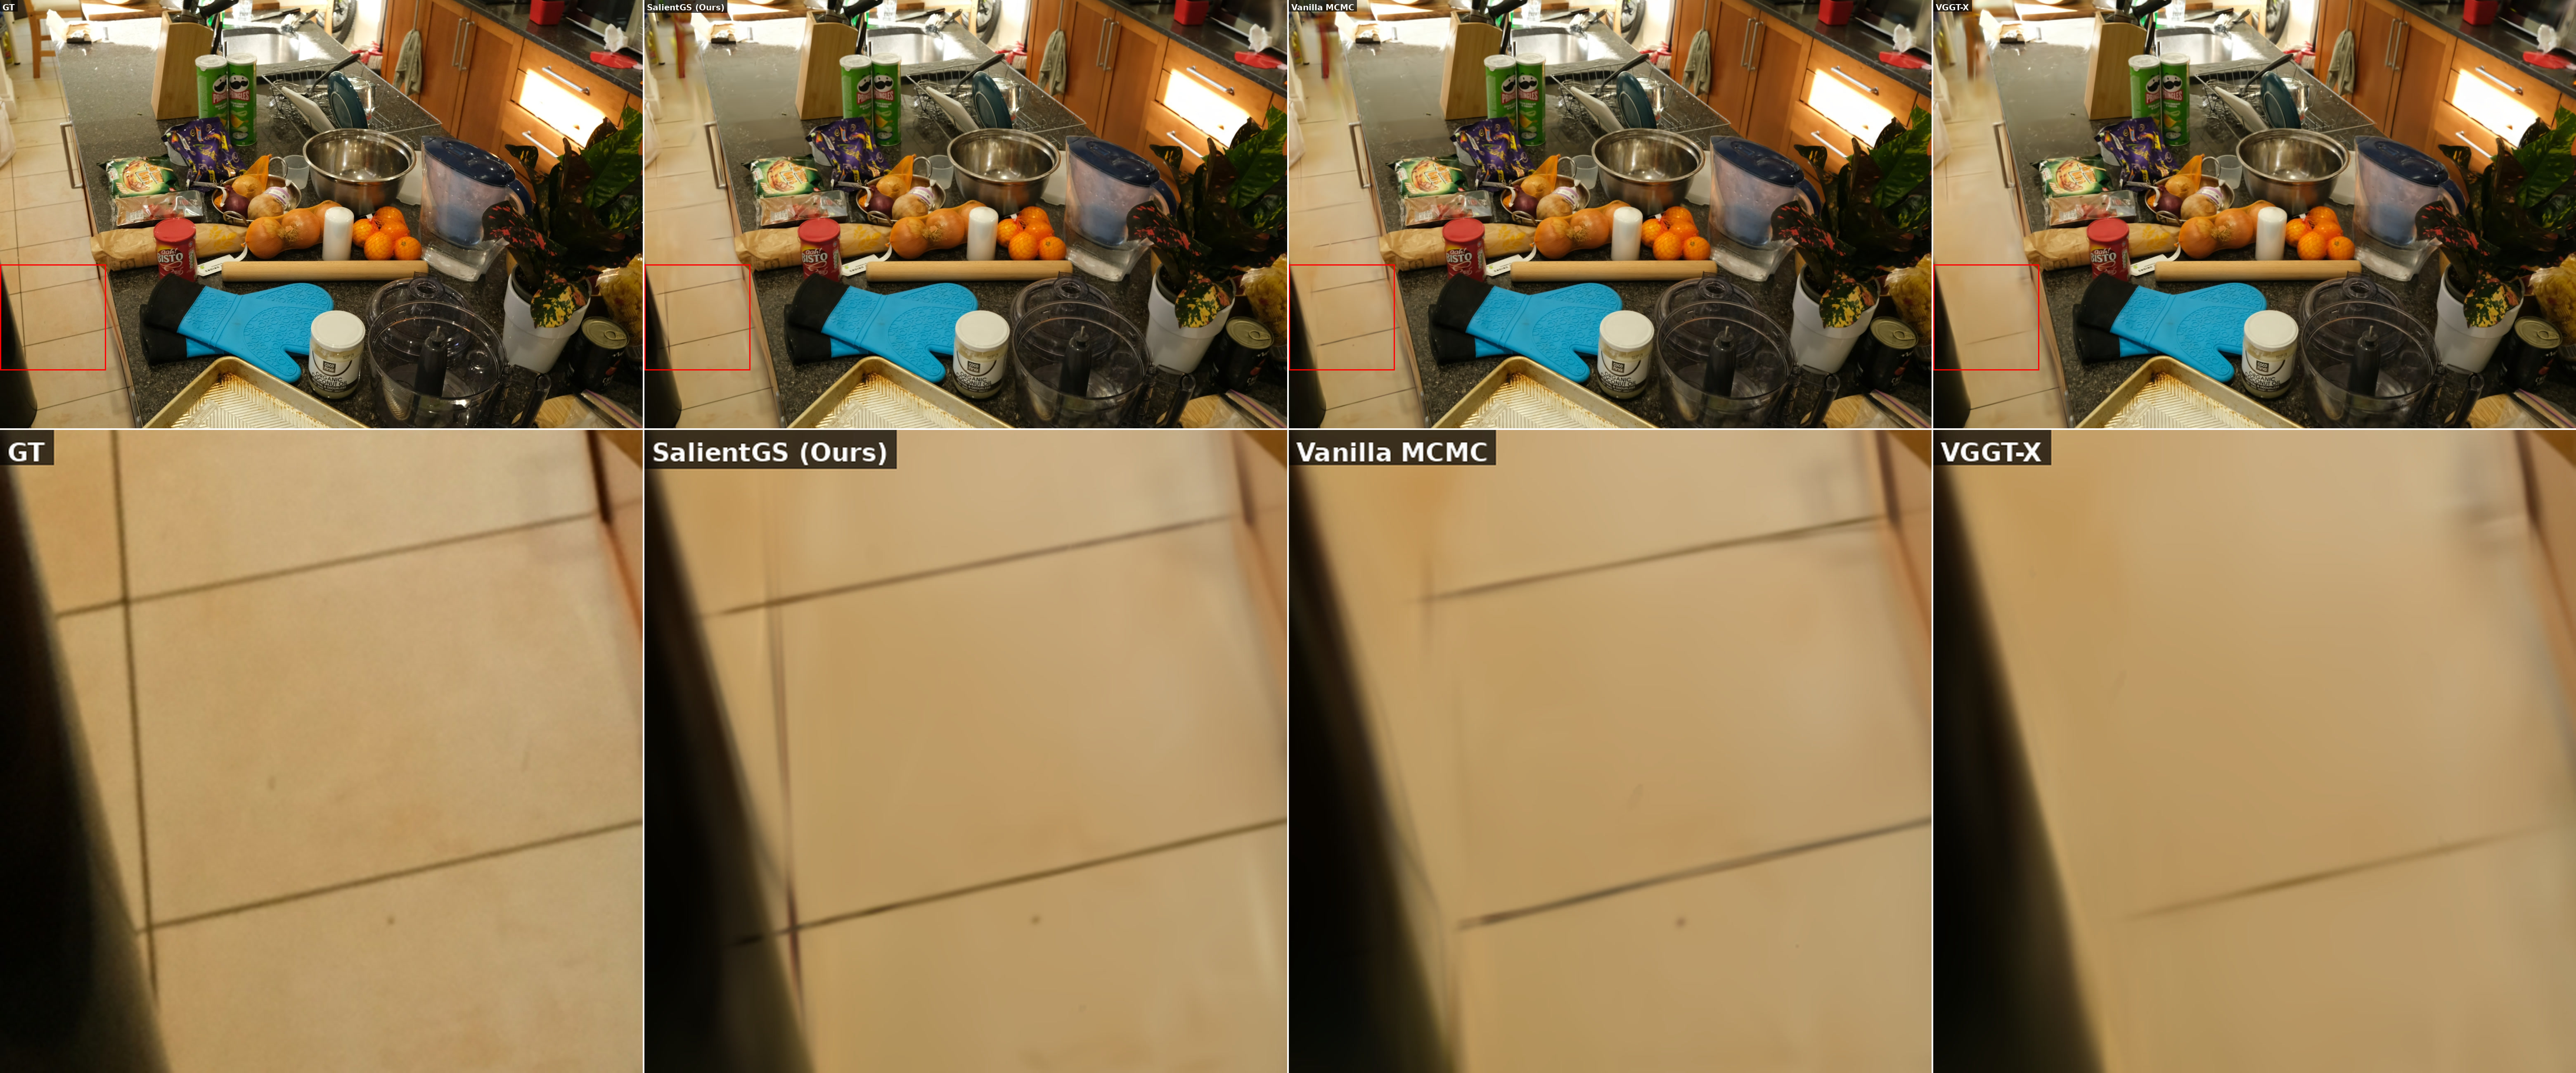
\includegraphics[width=\textwidth]{qualitative/qual_scene_counter.jpg}
    \caption{Per-scene qualitative comparison: \textit{counter}.}
    \label{fig:supp_counter}
\end{figure*}

\begin{figure*}[t]
    \centering
    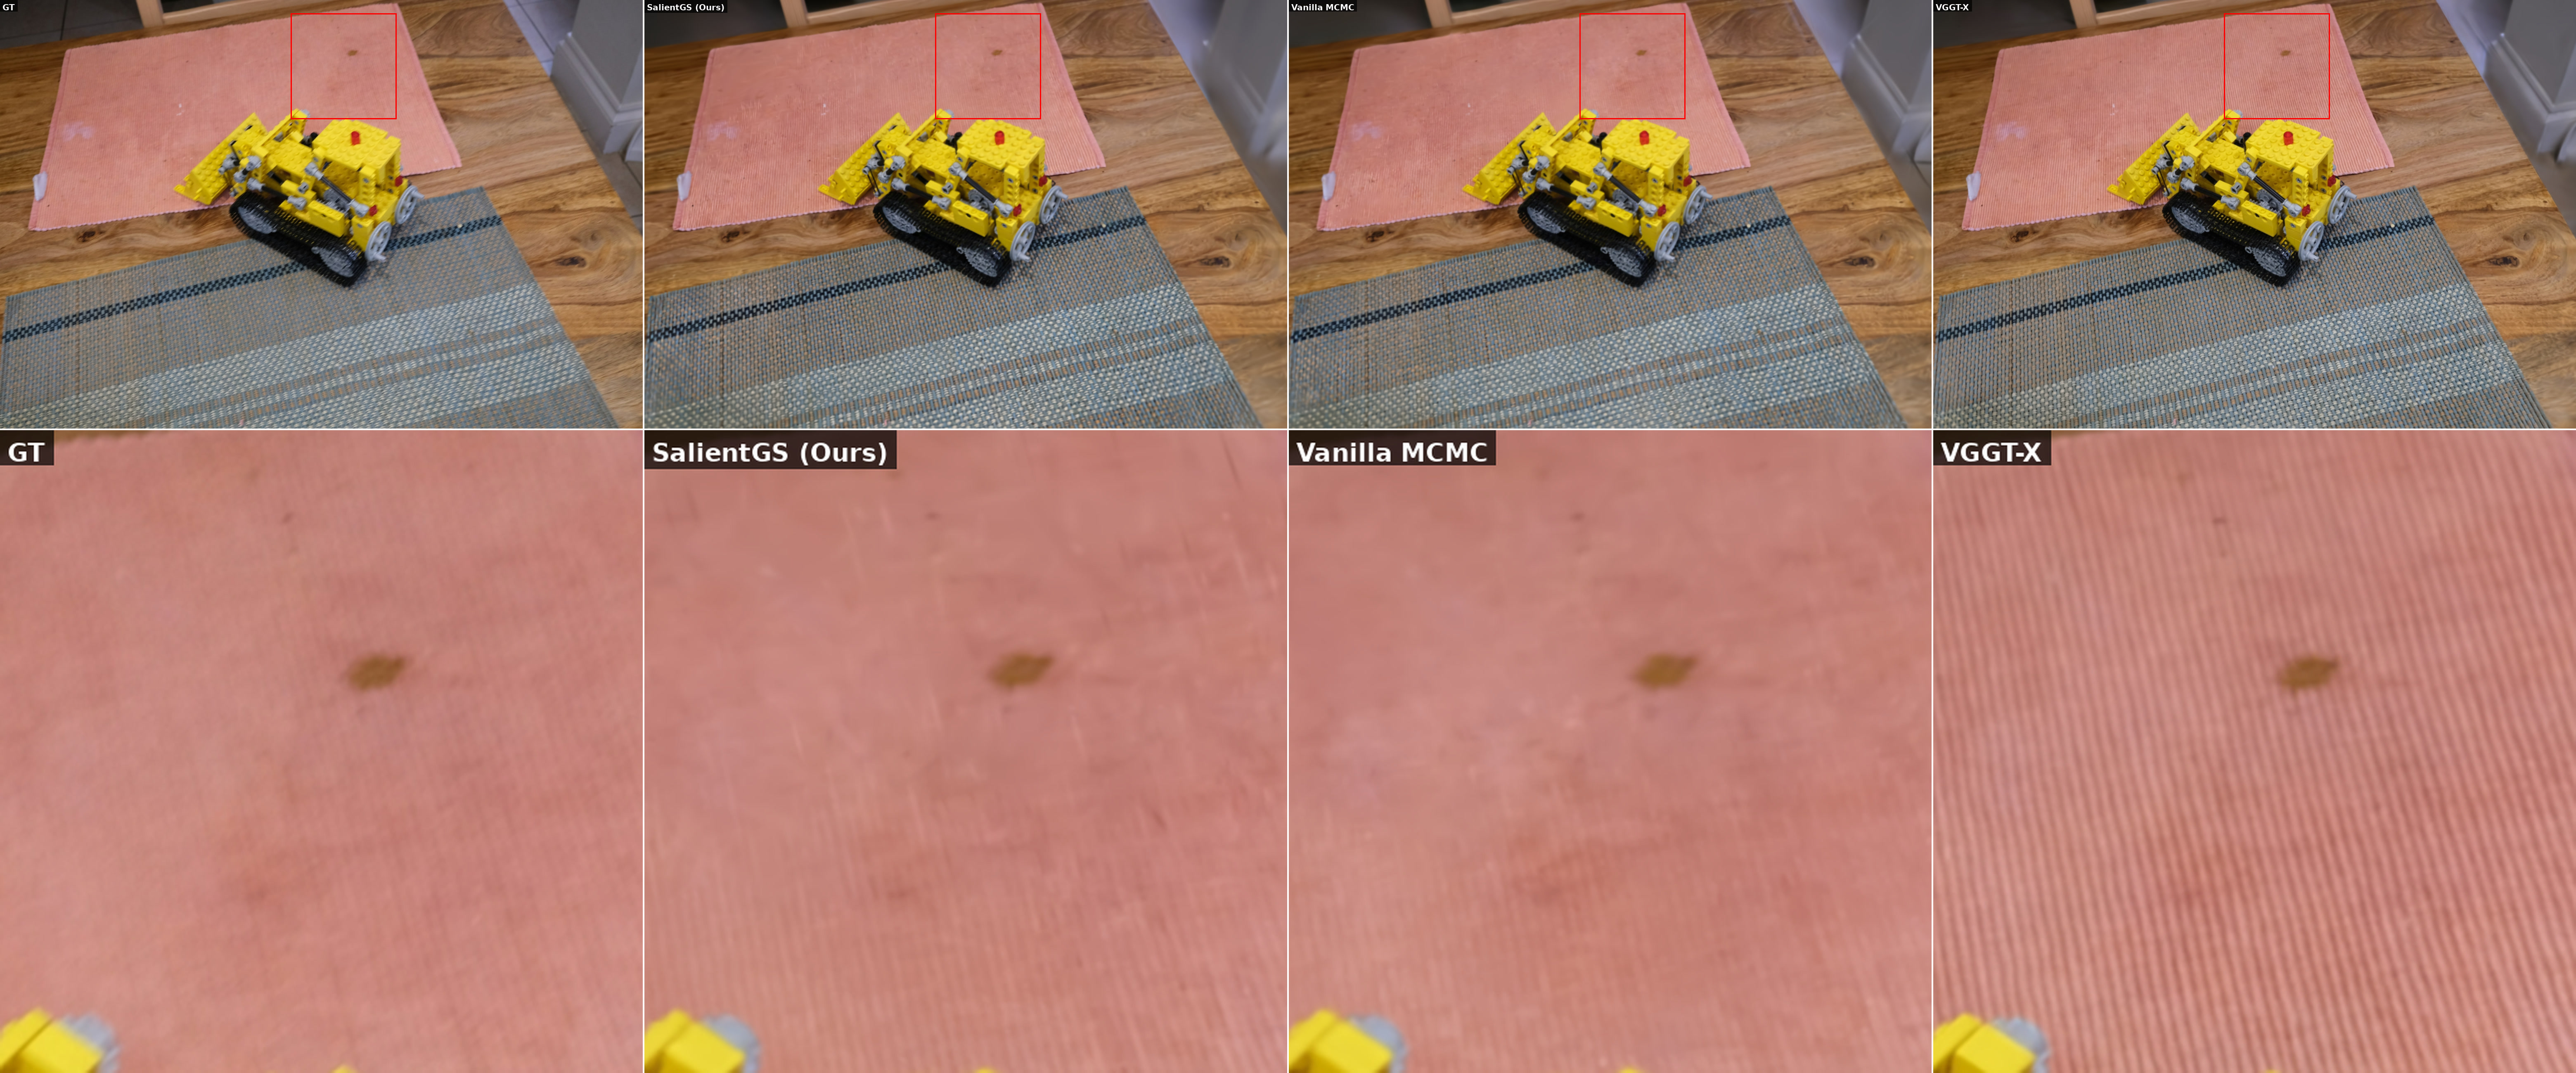
\includegraphics[width=\textwidth]{qualitative/qual_scene_kitchen.jpg}
    \caption{Per-scene qualitative comparison: \textit{kitchen}.}
    \label{fig:supp_kitchen}
\end{figure*}

\begin{figure*}[t]
    \centering
    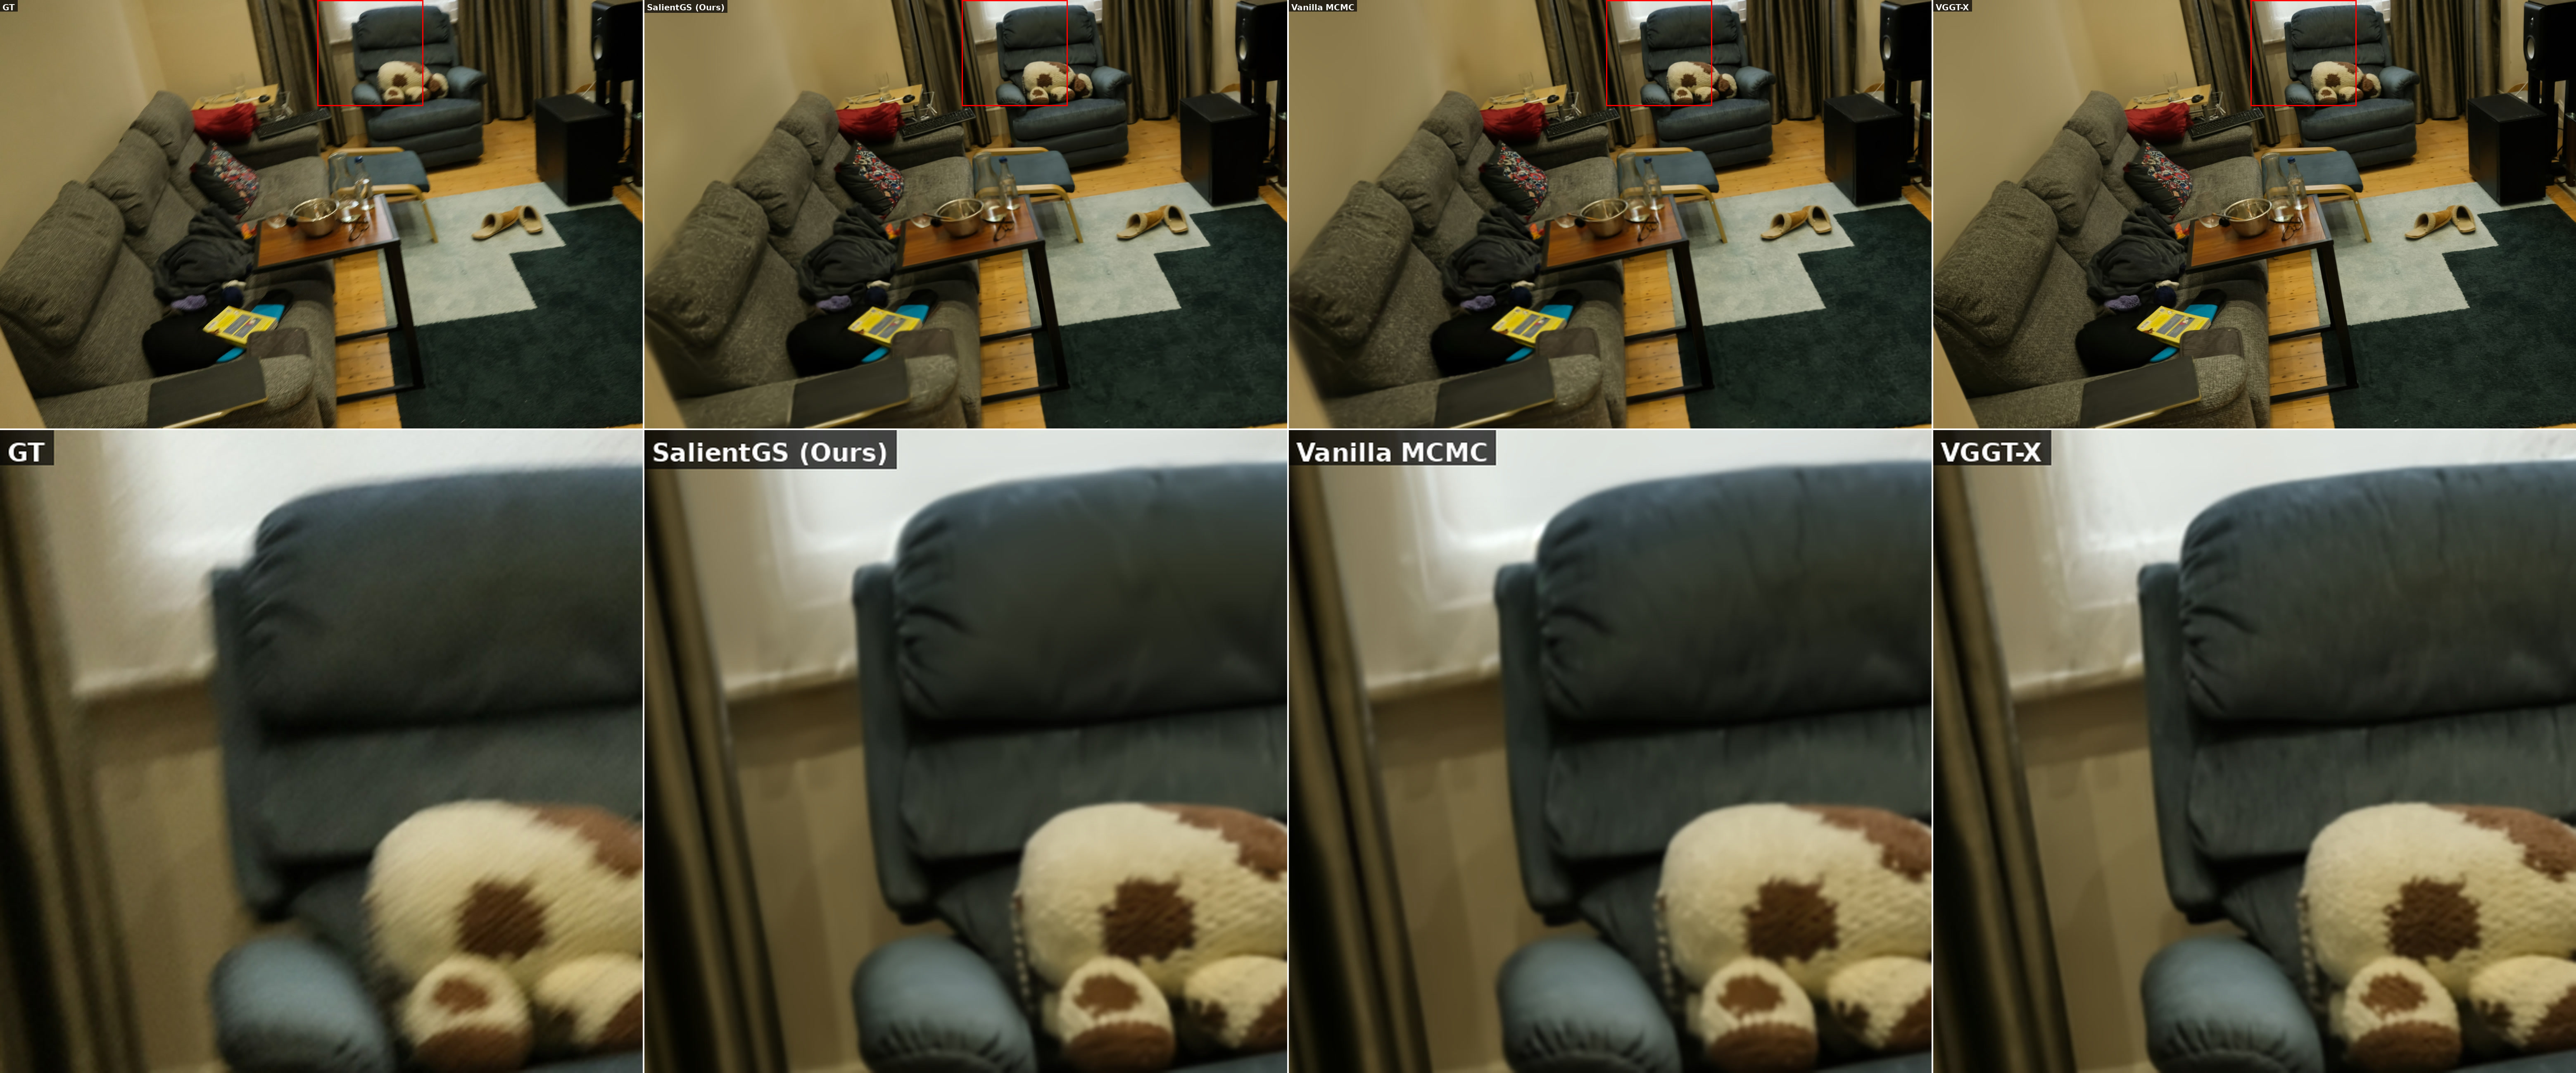
\includegraphics[width=\textwidth]{qualitative/qual_scene_room.jpg}
    \caption{Per-scene qualitative comparison: \textit{room}. SalientGS underperforms on this indoor scene with uniform textures, where first-order SfM provides weaker geometric constraints.}
    \label{fig:supp_room}
\end{figure*}

%% =============================================================================
%% Per-Image LPIPS Analysis
%% =============================================================================
\section{Per-Image LPIPS Analysis}
\label{sec:supp_per_image_lpips}

Table~\ref{tab:supp_per_scene_lpips} combines the released SalientGS verification with the controlled camera-ready ablation measurements. At full precision, SalientGS improves over vanilla MCMC on seven scenes and trails it on \textit{flowers} and \textit{counter}; \textit{garden} and \textit{treehill} appear tied after rounding. Its nine-scene mean is substantially lower (0.148 vs.\ 0.189). Because the columns come from two documented experiment snapshots, this table is descriptive; causal allocator conclusions are drawn from the matched controlled tables in \S\ref{sec:supp_camera_ready_ablations}.

\begin{table}[t]
    \centering
    \footnotesize
    \setlength\tabcolsep{3pt}
    \caption{
        \textbf{Mean per-image LPIPS ($\downarrow$) on Mip-NeRF 360 scenes.}
        Scene rows show per-scene means. We report both the scene-equal mean used in the main comparison and the pooled test-image diagnostic. Best displayed result per scene in \textbf{bold}.
    }
    \resizebox{\columnwidth}{!}{%
    \begin{tabular}{l cccc}
        \toprule
        Scene & SalientGS & Vanilla MCMC & Std.\ ADC & Freeze Poses \\
        \midrule
        \multicolumn{5}{l}{\textit{Outdoor Scenes}} \\
        \quad bicycle   & \textbf{0.135} & 0.152 & 0.153 & 0.173 \\
        \quad flowers   & 0.274 & \textbf{0.264} & 0.309 & 0.293 \\
        \quad garden    & 0.074 & 0.074 & \textbf{0.066} & 0.081 \\
        \quad stump     & \textbf{0.123} & 0.140 & 0.145 & 0.151 \\
        \quad treehill  & \textbf{0.260} & \textbf{0.260} & 0.269 & 0.270 \\
        \midrule
        \multicolumn{5}{l}{\textit{Indoor Scenes}} \\
        \quad bonsai    & \textbf{0.106} & 0.169 & 0.171 & 0.170 \\
        \quad counter   & 0.136 & \textbf{0.132} & 0.148 & 0.134 \\
        \quad kitchen   & \textbf{0.076} & 0.236 & 0.167 & 0.173 \\
        \quad room      & \textbf{0.150} & 0.271 & 0.252 & 0.271 \\
        \midrule
        \textbf{Scene mean}& \textbf{0.148} & 0.189 & 0.187 & 0.192 \\
        \textbf{Pooled images}& \textbf{0.140} & 0.189 & 0.187 & 0.191 \\
        \bottomrule
    \end{tabular}%
    }
    \label{tab:supp_per_scene_lpips}
\end{table}

%% =============================================================================
%% Threshold Sensitivity Sweep
%% =============================================================================
\section{Threshold Sensitivity Sweep}
\label{sec:supp_threshold}

Table~\ref{tab:supp_threshold} reports the Mip-NeRF 360 sensitivity sweep referenced in the main paper. We vary the importance threshold $\tau_{\text{imp}}$ and the number of views $K$ used for multi-view score computation while keeping the rest of the pipeline fixed.

The released setting uses $\tau_{\text{imp}}{=}5$ and $K{=}10$. PSNR and SSIM vary mildly across nearby settings, while LPIPS is more sensitive to perceptual blur and high-frequency detail; we therefore report the three metrics separately rather than summarizing robustness with a single PSNR range.

\begin{table}[t]
    \centering
    \footnotesize
    \setlength\tabcolsep{4pt}
    \caption{
        \textbf{Threshold-sensitivity sweep on Mip-NeRF 360.}
        We vary the importance threshold $\tau_{\text{imp}}$ and the number of scoring views $K$. The selected full-model configuration is marked as \emph{default}.
    }
    \resizebox{\columnwidth}{!}{%
    \begin{tabular}{l c ccc}
        \toprule
        Group & Value & PSNR$\uparrow$ & SSIM$\uparrow$ & LPIPS$\downarrow$ \\
        \midrule
        \multirow{5}{*}{$\tau_{\text{imp}}$}
        & 1  & 28.688 & 0.8444 & 0.159 \\
        & 3  & 28.685 & 0.8448 & 0.157 \\
        & 5 (\emph{default})  & \textbf{28.822} & \textbf{0.8531} & \textbf{0.148} \\
        & 10 & 28.732 & 0.8466 & 0.153 \\
        & 20 & 28.759 & 0.8477 & 0.151 \\
        \midrule
        \multirow{5}{*}{$K$}
        & 3  & 28.696 & 0.8457 & 0.156 \\
        & 5  & 28.689 & 0.8455 & 0.156 \\
        & 10 (\emph{default}) & \textbf{28.822} & \textbf{0.8531} & \textbf{0.148} \\
        & 15 & 28.714 & 0.8450 & 0.157 \\
        & 20 & 28.679 & 0.8446 & 0.157 \\
        \bottomrule
    \end{tabular}%
    }
    \label{tab:supp_threshold}
\end{table}

%% =============================================================================
%% Front-End Gap Analysis and Track-Length Ablation
%% =============================================================================
\section{Front-End Track Analysis and Track-Length Ablation}
\label{sec:supp_track_analysis}

A natural question is whether the quality advantage of SalientGS over retrieval-only front-ends (such as GloSplat-F, which uses XFeat+LightGlue with top-5 retrieval) originates primarily from better Gaussian allocation or from a richer multi-view track structure. We investigate this through two complementary experiments: (1)~a comparison of the 3D-point track-length distributions produced by three front-ends on the \texttt{bicycle} scene, and (2)~a controlled track-length cap ablation that holds the front-end fixed and varies only the maximum number of observations retained per track before global positioning and bundle adjustment.

\paragraph{Track-Length Distributions.}
Table~\ref{tab:track_dist} compares the track-length distributions produced on the \texttt{bicycle} scene by three pipelines: GloSplat-A (SIFT exhaustive), GloSplat-F (XFeat+LightGlue, retrieval top-5), and SalientGS (SIFT + Fisher Vector retrieval, $k{=}20$).
SalientGS reconstructs ${\sim}4\%$ fewer 3D points than GloSplat-A (51.8k vs.\ 54.3k), but its track-length distribution remains very close: median and max are nearly identical, the mean is only marginally lower (4.47 vs.\ 4.69), and all four length-bucket percentages differ by at most 0.6\,pp.
In contrast, GloSplat-F---which uses only 5 retrieval neighbors---yields ${\sim}16\%$ fewer points with a substantially shorter track distribution (median 3 vs.\ 4, max 20 vs.\ 74), and long tracks (${\ge}9$ observations) are nearly absent (2.1\% vs.\ 9.5\%).
The MST connectivity guarantee built into SalientGS's Fisher Vector retrieval (Sec.~3.1 of the main paper) is responsible for preserving the exhaustive-like track structure: the $k{=}20$ candidate graph, augmented with MST edges, achieves far denser coverage than a bare top-5 list.

\begin{table}[h]
\centering
\caption{Track-length distribution on the \texttt{bicycle} scene for GloSplat-A (SIFT exhaustive), GloSplat-F (XFeat+LightGlue, retrieval top-5), and SalientGS (Fisher Vector, $k{=}20$).}
\label{tab:track_dist}
\resizebox{\columnwidth}{!}{%
\begin{tabular}{lrrr}
\toprule
 & GloSplat-A & GloSplat-F & SalientGS \\
\midrule
Total points & 54{,}275 & 45{,}507 & 51{,}847 \\
Mean / Median & 4.69\,/\,4 & 3.75\,/\,3 & 4.47\,/\,4 \\
Max & 74 & 20 & 71 \\
\midrule
2--3  & 26{,}861 (49.5\%) & 27{,}182 (59.7\%) & 25{,}814 (49.8\%) \\
4--8  & 22{,}036 (40.6\%) & 17{,}366 (38.2\%) & 21{,}124 (40.7\%) \\
9--16 & 4{,}694\phantom{0} (8.6\%) & 948\phantom{00} (2.1\%) & 4{,}133\phantom{0} (8.0\%) \\
17+   & 684\phantom{00} (1.3\%) & 11\phantom{000} (0.0\%) & 776\phantom{00} (1.5\%) \\
\bottomrule
\end{tabular}%
}
\end{table}

\paragraph{Track-Length Cap Ablation.}
To establish causality between track length and downstream rendering quality, we conduct a controlled ablation: we fix each method's front-end (i.e., the same pair graph and matches) and vary only the maximum number of observations retained per track before global positioning and bundle adjustment. Table~\ref{tab:track_cap} reports the effect on Mip-NeRF 360 (averaged over 9 scenes).
The $L{=}2$ condition reduces every track to a pairwise observation---simulating a worst-case version of the track shortening seen in GloSplat-F---while $L{=}\text{all}$ retains the full distribution.
For GloSplat (SIFT exhaustive front-end), capping at $L{=}2$ causes a 1.40\,dB PSNR drop (28.86\,$\to$\,27.46), confirming that long multi-view tracks provide substantial geometric constraints that improve triangulation robustness and stabilize bundle adjustment.
In the matched track-cap experiment, SalientGS exhibits a similar degradation of 1.29\,dB (28.82\,$\to$\,27.53) under the same $L{=}2$ cap. Once every track is reduced to a pairwise observation, both pipelines operate on geometrically equivalent constraints regardless of their front-end or allocation strategy, leaving the underlying bundle adjustment quality as the dominant factor.

\begin{table}[t]
\centering
\caption{Track-length cap ablation on MipNeRF360 (9-scene avg.). The front-end is fixed for each method; only the maximum retained observations per track varies.}
\label{tab:track_cap}
\resizebox{\columnwidth}{!}{%
\begin{tabular}{lccc}
\toprule
Max track length & PSNR\,$\uparrow$ & SSIM\,$\uparrow$ & LPIPS\,$\downarrow$ \\
\midrule
\multicolumn{4}{l}{\textit{GloSplat (SIFT exhaustive front-end)}} \\
\quad \textit{GloSplat-F (retrieval top-5, ref.)} & \textit{27.77} & \textit{0.818} & \textit{0.164} \\
\quad $L = 2$          & 27.46 & 0.804 & 0.174 \\
\quad $L = \text{all}$ & 28.86 & 0.862 & 0.139 \\
\quad \textit{GloSplat-A (exhaustive, ref.)}  & \textit{28.86} & \textit{0.862} & \textit{0.139} \\
\midrule
\multicolumn{4}{l}{\textit{SalientGS (Fisher Vector $k{=}20$ front-end)}} \\
\quad $L = 2$          & 27.53 & 0.808 & 0.172 \\
\quad $L = \text{all}$ (full model) & \textbf{28.82} & \textbf{0.853} & \textbf{0.148} \\
\bottomrule
\end{tabular}%
}
\end{table}

\noindent Taken together, these results support two conclusions. First, SalientGS's Fisher Vector retrieval with $k{=}20$ and MST connectivity is sufficient to recover an exhaustive-quality track distribution at a fraction of the matching cost, closing the structural gap that limits GloSplat-F. Second, the near-identical $L{=}2$ scores across both methods confirm that the gain from full tracks is a property of multi-view triangulation geometry, not of any particular front-end or allocation design---making rich track coverage a necessary condition for high-quality reconstruction.

%% =============================================================================
%% Additional camera-ready experiments from the rebuttal
%% =============================================================================
\section{Additional Camera-Ready Ablations}
\label{sec:supp_camera_ready_ablations}

This section records the ablations completed during the author response. All occurrences of the complete default model use the corrected released aggregate, 28.82~dB / 0.853 / 0.148; the remaining variant measurements are unchanged.

\begin{table*}[t]
    \centering
    \caption{SfM initialization versus Gaussian allocator on Mip-NeRF 360. All rows use the same joint training protocol.}
    \label{tab:supp_init_allocator}
    \begin{tabular}{l lccc}
        \toprule
        SfM initialization & Allocator & PSNR$\uparrow$ & SSIM$\uparrow$ & LPIPS$\downarrow$ \\
        \midrule
        GLOMAP & ADC & 27.52 & 0.827 & 0.168 \\
        GLOMAP & Vanilla MCMC & 28.70 & 0.846 & 0.151 \\
        GLOMAP & Guided MCMC & \textbf{28.87} & \textbf{0.855} & \textbf{0.133} \\
        FastMap & ADC & 27.67 & 0.828 & 0.162 \\
        FastMap & Vanilla MCMC & 28.72 & 0.848 & 0.149 \\
        FastMap & Guided MCMC (full model) & 28.82 & 0.853 & 0.148 \\
        \bottomrule
    \end{tabular}
\end{table*}

Table~\ref{tab:supp_init_allocator} shows that guided allocation improves both initializers: LPIPS changes from 0.151 to 0.133 for GLOMAP and from 0.149 to 0.148 for FastMap. This supports an allocator contribution that is not specific to one camera initializer.

\begin{table}[t]
    \centering
    \footnotesize
    \caption{Importance-score schedule and opacity mixing on Mip-NeRF 360.}
    \label{tab:supp_schedule}
    \begin{tabular}{lccc}
        \toprule
        Setting & PSNR$\uparrow$ & SSIM$\uparrow$ & LPIPS$\downarrow$ \\
        \midrule
        $T=100$ & 28.83 & 0.855 & 0.135 \\
        $T=200$ & \textbf{28.87} & \textbf{0.856} & \textbf{0.133} \\
        $T=500$ (default/full) & 28.82 & 0.853 & 0.148 \\
        $T=1000$ & 28.80 & 0.852 & 0.137 \\
        \midrule
        score at iter. 0 & 28.78 & 0.851 & \textbf{0.138} \\
        score at iter. 3000 (default/full) & \textbf{28.82} & \textbf{0.853} & 0.148 \\
        \midrule
        $\lambda_{\rm mix}=0$ & 28.78 & 0.851 & \textbf{0.141} \\
        $\lambda_{\rm mix}=0.05$ (default/full) & \textbf{28.82} & \textbf{0.853} & 0.148 \\
        $\lambda_{\rm mix}=0.20$ & 28.75 & 0.850 & 0.145 \\
        \bottomrule
    \end{tabular}
\end{table}

\begin{table}[t]
    \centering
    \footnotesize
    \caption{Robust quantile normalization and selection-quantile interaction on Mip-NeRF 360. The final row reports the fraction of Gaussians in the high-error mass at 30K iterations.}
    \label{tab:supp_quantiles}
    \begin{tabular}{lccc}
        \toprule
        Setting & PSNR$\uparrow$ & SSIM$\uparrow$ & LPIPS$\downarrow$ \\
        \midrule
        Plain min--max & 28.71 & 0.850 & 0.150 \\
        Default quantiles (full) & \textbf{28.82} & \textbf{0.853} & 0.148 \\
        $(q_{\rm hi},q_{\rm lo})=(.80,.20)$ & 28.79 & 0.852 & 0.139 \\
        $(q_{\rm hi},q_{\rm lo})=(.95,.05)$ & \textbf{28.82} & 0.851 & \textbf{0.137} \\
        High-error mass at 30K & \multicolumn{3}{c}{robust: 9.1\%; min--max: 42.5\%} \\
        \bottomrule
    \end{tabular}
\end{table}

\begin{table}[t]
    \centering
    \footnotesize
    \caption{Pose error before and after joint optimization on the ETH3D SLAM evaluation. Errors are in centimeters; percentages are fractions of cameras below the indicated threshold.}
    \label{tab:supp_pose_errors}
    \begin{tabular}{lrrrr}
        \toprule
        Method & Median$\downarrow$ & Mean$\downarrow$ & $<5$cm$\uparrow$ & $<10$cm$\uparrow$ \\
        \midrule
        FastMap init & 9.8 & 18.5 & 31.6 & 50.5 \\
        FastMap + joint & \textbf{6.9} & 13.5 & \textbf{38.2} & \textbf{57.0} \\
        GLOMAP init & 8.5 & 14.6 & 35.5 & 55.5 \\
        GLOMAP + joint & 7.1 & \textbf{12.6} & 37.8 & 56.5 \\
        \bottomrule
    \end{tabular}
\end{table}

\begin{table}[t]
    \centering
    \footnotesize
    \caption{Per-scene Deep Blending results. The competing methods fail on \textit{drjohnson}, which explains the averaged values in the main table.}
    \label{tab:supp_deep_blending_split}
    \begin{tabular}{llrrr}
        \toprule
        Scene & Method & PSNR$\uparrow$ & SSIM$\uparrow$ & LPIPS$\downarrow$ \\
        \midrule
        \textit{playroom} & GloSplat-A & 29.38 & 0.903 & 0.224 \\
        \textit{playroom} & SalientGS & \textbf{30.15} & \textbf{0.920} & \textbf{0.156} \\
        \textit{drjohnson} & GloSplat-A & 7.52 & 0.263 & 0.792 \\
        \textit{drjohnson} & VGGT-X & 7.65 & 0.337 & 0.858 \\
        \textit{drjohnson} & SalientGS & \textbf{28.82} & \textbf{0.892} & \textbf{0.210} \\
        \bottomrule
    \end{tabular}
\end{table}

\begin{table}[t]
    \centering
    \footnotesize
    \caption{Budget efficiency on Mip-NeRF 360.}
    \label{tab:supp_budget}
    \begin{tabular}{rccc}
        \toprule
        $\mathrm{N_{GS}}$ & Vanilla MCMC & Guided MCMC & $\Delta$PSNR \\
        \midrule
        500K & 28.19 & 28.46 & +0.27 \\
        1.0M & 28.59 & 28.81 & +0.22 \\
        1.5M & 28.72 & 28.82 & +0.10 \\
        2.0M & 28.80 & 28.93 & +0.13 \\
        3.0M & 28.88 & 28.97 & +0.09 \\
        \bottomrule
    \end{tabular}
\end{table}

\section{Additional Robustness and Failure Diagnostics}
\label{sec:supp_robustness}

\begin{table}[t]
    \centering
    \footnotesize
    \caption{Dense indoor robustness. SG denotes SalientGS and V+M denotes the VGGT-X+MCMC comparison.}
    \label{tab:supp_indoor}
    \begin{tabular}{lrrrr}
        \toprule
        Scene & SG PSNR & V+M PSNR & SG LPIPS & V+M LPIPS \\
        \midrule
        bonsai & 33.21 & 30.71 & 0.106 & 0.139 \\
        counter & 29.60 & 28.80 & 0.136 & 0.158 \\
        kitchen & 32.79 & 29.68 & 0.076 & 0.113 \\
        room & 31.95 & 30.76 & 0.150 & 0.165 \\
        Average & \textbf{31.89} & 29.99 & \textbf{0.117} & 0.144 \\
        \bottomrule
    \end{tabular}
\end{table}

\begin{table}[t]
    \centering
    \footnotesize
    \caption{Additional large-scene and drone-capture evidence.}
    \label{tab:supp_large_scene_summary}
    \resizebox{\columnwidth}{!}{%
    \begin{tabular}{ll}
        \toprule
        Setting & Result \\
        \midrule
        Mill-19 Building & Best PSNR, 24.19~dB \\
        Mill-19 Rubble & Best PSNR, 26.98~dB \\
        Four large scenes & Best PSNR/LPIPS on 3 of 4 scenes \\
        Runtime/memory & $\sim$1~h / $\sim$5~GB vs. $\sim$3~h / $\sim$14~GB for CityGS-X \\
        \bottomrule
    \end{tabular}%
    }
\end{table}

\begin{table}[t]
    \centering
    \footnotesize
    \caption{Failure diagnostics and fallback on representative Mip-NeRF 360 scenes. Residual is the normalized early epipolar residual.}
    \label{tab:supp_failure}
    \resizebox{\columnwidth}{!}{%
    \begin{tabular}{lrrrr}
        \toprule
        Scene & Median track & Mean degree & MST reliance & Residual \\
        \midrule
        garden & 4 & 18.4 & 4\% & 0.20 \\
        kitchen & 3 & 13.4 & 11\% & 0.43 \\
        room & 2 & 9.7 & 21\% & 0.57 \\
        \midrule
        \multicolumn{5}{l}{\textit{room LPIPS: original 0.312; fallback 0.235; VGGT-X 0.244}} \\
        \bottomrule
    \end{tabular}%
    }
\end{table}

The diagnostics in Table~\ref{tab:supp_failure} identify the texture-poor \textit{room} case through collapsed track length, greater MST reliance, and a high early residual. A feed-forward fallback improves the failure-view LPIPS from 0.312 to 0.235, slightly better than the VGGT-X reference of 0.244. Sparse/few-view reconstruction and severe repetitive or symmetric appearance remain limitations; learned retrieval and adaptive geometry-aware budgets are natural future extensions.

\begin{table}[t]
    \centering
    \footnotesize
    \caption{Sequential Tanks \& Temples comparison with CF-3DGS.}
    \label{tab:supp_cf3dgs}
    \begin{tabular}{llrrr}
        \toprule
        Scene & Method & PSNR$\uparrow$ & SSIM$\uparrow$ & LPIPS$\downarrow$ \\
        \midrule
        Family & CF-3DGS & 33.12 & 0.960 & 0.051 \\
        Family & SalientGS & \textbf{36.80} & \textbf{0.970} & \textbf{0.024} \\
        Francis & CF-3DGS & 32.78 & 0.915 & 0.135 \\
        Francis & SalientGS & \textbf{36.29} & \textbf{0.947} & \textbf{0.056} \\
        \bottomrule
    \end{tabular}
\end{table}

%% =============================================================================
%% BIBLIOGRAPHY
%% =============================================================================
\clearpage
\bibliographystyle{ACM-Reference-Format}
\bibliography{references}

\end{document}
